
\documentclass[usenames,dvipsnames]{beamer}
%\includeonlyframes{current} Does not work, though
\mode<presentation>{
\usefonttheme{professionalfonts}
\useinnertheme{rounded}
\useoutertheme[subsection=false,footline=authortitle]{miniframes}
%Inner Color Themes
\usecolortheme{dolphin}
%	\usecolortheme{seahorse}


%Outer Color Themes
\usecolortheme{rose}
%\usecolortheme{orchid}
}

%Typical documenttypes: article/book
%some examples:
%\documentclass[reqno,11pt]{book}   %%%for books
%\documentclass[]{minimal}			%%%for Minimal Working Example






%%%%%%%%%%%%%%%%%%%% setting for fast compiling

%\special{dvipdfmx:config z 0}		% no compression

\includeonly{chapters/chapter9}		% In practice, use an empty document called "chapter9"	% usually for printing books






%%%%%%%%%%%%%%%%%%%% here we include packages

%%%basic packages for math articles
\usepackage{amssymb}
\usepackage{amsthm}
\usepackage{amsmath}
\usepackage{amsfonts}
%\usepackage[shortlabels]{enumitem}	% It supersedes both enumerate and mdwlist. The package option shortlabels is included to configure the labels like in enumerate.

%%%packages for special symbols
\usepackage{pifont}					% Access to PostScript standard Symbol and Dingbats fonts
\usepackage{wasysym}				% additional characters
\usepackage{bm}						% bold fonts: \bm{...}
\usepackage{extarrows}				% may be replaced by tikz-cd
%\usepackage{unicode-math}			% unicode maths for math fonts, now I don't know how to include it

%%%basic packages for fancy electronic documents
%\usepackage[colorlinks]{hyperref}
%\usepackage[table,hyperref]{xcolor} 			% before tikz-cd. 
%\usepackage[table,hyperref,monochrome]{xcolor}	% disable colored output (black and white)

%%%packages for figures and tables (general setting)
\usepackage{float}				%Improved interface for floating objects
\usepackage{caption,subcaption}
\usepackage{adjustbox}			% for me it is usually used in tables 
\usepackage{stackengine}		%baseline changes

%%%packages for commutative diagrams
\usepackage{tikz-cd}
\usepackage{quiver}			% see https://q.uiver.app/

%%%packages for pictures
\usepackage[width=0.5,tiewidth=0.7]{strands}
\usepackage{graphicx}			% Enhanced support for graphics

%%%packages for tables and general settings
\usepackage{array}
\usepackage{makecell}
\usepackage{multicol}
\usepackage{multirow}
\usepackage{diagbox}



%%%packages for temporary usage
\usepackage{mathtools}
\usepackage{tabularx}
\usepackage{etoolbox}



%https://tex.stackexchange.com/questions/58852/possible-incompatibility-with-enumitem










%%%%%%%%%%%%%%%%%%%% here we include theoremstyles

\numberwithin{equation}{section}

\theoremstyle{plain}
%\newtheorem{theorem}{Theorem}[section]

\newtheorem{setting}[theorem]{Setting}
%\newtheorem{definition}[theorem]{Definition}
%\newtheorem{lemma}[theorem]{Lemma}
\newtheorem{proposition}[theorem]{Proposition}
%\newtheorem{corollary}[theorem]{Corollary}
\newtheorem{conjecture}[theorem]{Conjecture}

\newtheorem{claim}[theorem]{Claim}
\newtheorem{eg}[theorem]{Example}
\newtheorem{ex}[theorem]{Exercise}
%\newtheorem{fact}[theorem]{Fact}
\newtheorem{ques}[theorem]{Question}
\newtheorem{warning}[theorem]{Warning}



\newtheorem*{bbox}{Black box}
\newtheorem*{notation}{Conventions and Notations}


\numberwithin{equation}{section}


\theoremstyle{remark}

\newtheorem{remark}[theorem]{Remark}
\newtheorem*{remarks}{Remarks}

%%% for important theorems
%\newtheoremstyle{theoremletter}{4mm}{1mm}{\itshape}{ }{\bfseries}{}{ }{}
%\theoremstyle{theoremletter}
%\newtheorem{theoremA}{Theorem}
%\renewcommand{\thetheoremA}{A}
%\newtheorem{theoremB}{Theorem}
%\renewcommand{\thetheoremB}{B}

\newtheorem{short}{ }





%%%%%%%%%%%%%%%%%%%% here we declare some symbols

%%%%%%%DeclareMathOperator
%see here for why newcommand is better for DeclareMathOperator: https://tex.stackexchange.com/questions/67506/newcommand-vs-declaremathoperator

%%%%%basic symbols. Keep them!

%%%symbols for sets and maps
\DeclareMathOperator{\pt}{\{\ast\}}	%points. Other possibilities are \{pt\}, \{*\}...
\DeclareMathOperator{\Id}{\operatorname{Id}}	%identity in groups.
\DeclareMathOperator{\Img}{\operatorname{Im}}

\DeclareMathOperator{\Ob}{\operatorname{Ob}}
\DeclareMathOperator{\Mor}{\operatorname{Mor}}	%difference of Mor and Hom: Hom is usually for abelian categories
\DeclareMathOperator{\Hom}{\operatorname{Hom}}	\DeclareMathOperator{\End}{\operatorname{End}}
\DeclareMathOperator{\Aut}{\operatorname{Aut}}

%%%symbols for linear algebras and 
%%linear algebras
\DeclareMathOperator{\tr}{\operatorname{tr}}
\DeclareMathOperator{\diag}{\operatorname{diag}}	%for diagonal matrices

%%abstract algebras
\DeclareMathOperator{\ord}{\operatorname{ord}}
\DeclareMathOperator{\gr}{\operatorname{gr}}
\DeclareMathOperator{\Frac}{\operatorname{Frac}}

%%%symbols for basic geometries
\DeclareMathOperator{\vol}{\operatorname{vol}}	%volume
\DeclareMathOperator{\dist}{\operatorname{dist}}
\DeclareMathOperator{\supp}{\operatorname{supp}}

%%%symbols for category
%%names of categories
\DeclareMathOperator{\Mod}{\operatorname{Mod}}
\DeclareMathOperator{\Vect}{\operatorname{Vect}}
\DeclareMathOperator{\rep}{\operatorname{rep}} %usually rep means the category of finite dimensional representations, while Rep means the category of representations.
\DeclareMathOperator{\Rep}{\operatorname{Rep}}


%%%symbols for homological algebras
\DeclareMathOperator{\Tor}{\operatorname{Tor}}
\DeclareMathOperator{\Ext}{\operatorname{Ext}}
\DeclareMathOperator{\gldim}{\operatorname{gl.dim}}
\DeclareMathOperator{\projdim}{\operatorname{proj.dim}}
\DeclareMathOperator{\injdim}{\operatorname{inj.dim}}
\DeclareMathOperator{\rad}{\operatorname{rad}}


%%%symbols for algebraic groups
\DeclareMathOperator{\GL}{\operatorname{GL}}
\DeclareMathOperator{\SL}{\operatorname{SL}}

%%%symbols for typical varieties
\DeclareMathOperator{\Gr}{\operatorname{Gr}}
\DeclareMathOperator{\Flag}{\operatorname{Flag}}

%%%symbols for basic algebraic geometry
\DeclareMathOperator{\Spec}{\operatorname{Spec}}
\DeclareMathOperator{\Coh}{\operatorname{Coh}}
\newcommand{\Dcoh}{\mathcal{D}_{\operatorname{Coh}}}%%%This one shows the difference between \DeclareMathOperator and \newcommand
\DeclareMathOperator{\Pic}{\operatorname{Pic}}
\DeclareMathOperator{\Jac}{\operatorname{Jac}}

%%%%%advanced symbols. Choose the part you need!

%%%symbols for algebraic representation theory
\DeclareMathOperator{\Irr}{\operatorname{Irr}}
\DeclareMathOperator{\ind}{\operatorname{ind}}	%\ind(Q) means the set of  equivalence classes of finite dimensional indecomposable representations
\DeclareMathOperator{\Res}{\operatorname{Res}}
\DeclareMathOperator{\Ind}{\operatorname{Ind}}
\DeclareMathOperator{\cInd}{\operatorname{c-Ind}}


%%%symbols for algebraic topology
\DeclareMathOperator{\EGG}{\operatorname{E}\!}
\DeclareMathOperator{\BGG}{\operatorname{B}\!}

\DeclareMathOperator{\chern}{\operatorname{ch}^{*}}
\DeclareMathOperator{\Td}{\operatorname{Td}}
\DeclareMathOperator{\AS}{\operatorname{AS}}	%Atiyah--Segal completion theorem 

%%%symbols for Auslander--Reiten theory 
\DeclareMathOperator{\Modup}{\overline{\operatorname{mod}}}
\DeclareMathOperator{\Moddown}{\underline{\operatorname{mod}}}
\DeclareMathOperator{\Homup}{\overline{\operatorname{Hom}}}
\DeclareMathOperator{\Homdown}{\underline{\operatorname{Hom}}}


%%%symbols for operad
\DeclareMathOperator{\Com}{\operatorname{\mathcal{C}om}}
\DeclareMathOperator{\Ass}{\operatorname{\mathcal{A}ss}}
\DeclareMathOperator{\Lie}{\operatorname{\mathcal{L}ie}}
\DeclareMathOperator{\calEnd}{\operatorname{\mathcal{E}nd}} %cal=\mathcal


%%%%%personal symbols. Use at your own risk!

%%%symbols only for master thesis
\DeclareMathOperator{\ptt}{\operatorname{par}}	%the partition map
\DeclareMathOperator{\str}{\operatorname{str}}	%strict case
\DeclareMathOperator{\RRep}{\widetilde{\operatorname{Rep}}}
\DeclareMathOperator{\Rpt}{\operatorname{R}}
\DeclareMathOperator{\Rptc}{\operatorname{\mathcal{R}}}
\DeclareMathOperator{\Spt}{\operatorname{S}}
\DeclareMathOperator{\Sptc}{\operatorname{\mathcal{S}}}
\DeclareMathOperator{\Kcurl}{\operatorname{\mathcal{K}}}
\DeclareMathOperator{\Hcurl}{\operatorname{\mathcal{H}}}
\DeclareMathOperator{\eu}{\operatorname{eu}}
\DeclareMathOperator{\Eu}{\operatorname{Eu}}
\DeclareMathOperator{\dimv}{\operatorname{\underline{\mathbf{dim}}}}
\DeclareMathOperator{\St}{\mathcal{Z}}

%%%%%symbols which haven't been classified. Add your own math operators here!


\DeclareMathOperator{\Modr}{\operatorname{-Mod}}
\DeclareMathOperator{\BM}{\operatorname{BM}}




%%%%%%%newcommand

%%%basic symbols
\newcommand{\norm}[1]{\Vert{#1}\Vert}

%%%symbols only for master thesis
\newcommand{\dimvec}[1]{\mathbf{#1}}
\newcommand{\abdimvec}[1]{|\dimvec{#1}|}
\newcommand{\ftdimvec}[1]{\underline{\dimvec{#1}}}

\newcommand{\absgp}[1]{\mathbb{#1}}
\newcommand{\WWd}{\absgp{W}_{\abdimvec{d}}}
\newcommand{\Wd}{W_{\dimvec{d}}}
\newcommand{\ww}{\varpi}
\newcommand{\MinWd}{\operatorname{Min}(\absgp{W}_{\abdimvec{d}},W_{\dimvec{d}})}
\newcommand{\Compd}{\operatorname{Comp}_{\dimvec{d}}}
\newcommand{\Shuffled}{\operatorname{Shuffle}_{\dimvec{d}}}


\newcommand{\Omcell}{\Omega}
\newcommand{\OOmcell}{\boldsymbol{\Omega}}
\newcommand{\Vcell}{\mathcal{V}}
\newcommand{\VVcell}{\boldsymbol{\mathcal{V}}}
\newcommand{\Ocell}{\mathcal{O}}
\newcommand{\OOcell}{\boldsymbol{\mathcal{O}}}
\newcommand{\preimage}[1]{\widetilde{#1}}
\newcommand{\orde}{\operatorname{ord}_e}
\newcommand{\fakestar}{*}

%as the subscription of Hom
\newcommand{\Alggp}{\text{-Alg gp}}


%%%%%symbols which haven't been determined. Add your own math operators here!
\newcommand{\Flagbra}[1]{\Flag_{(#1)}}



%%%%%%%%%%%%%%%%%%%% here we make some blocks for special features. 

%%%% todo notes %%%%
\usepackage[colorinlistoftodos,textsize=footnotesize]{todonotes}
\setlength{\marginparwidth}{2.5cm}
\newcommand{\leftnote}[1]{\reversemarginpar\marginnote{\footnotesize #1}}
\newcommand{\rightnote}[1]{\normalmarginpar\marginnote{\footnotesize #1}\reversemarginpar}


%%%% Show outline around overlayarea %%%%
%https://tex.stackexchange.com/questions/573822/show-outline-around-overlayarea
\makeatletter
\newif\ifbeamer@show@overlayarea
\pgfkeys{/beamer/overlayarea/.cd,show frame/.is if=beamer@show@overlayarea,
show frame/.default=true}
\beamer@show@overlayareafalse
\mode
<presentation>
{\renewenvironment{overlayarea}[3][]{%
  \pgfkeys{/beamer/overlayarea/.cd,#1}%
  \beamer@animht=#2\relax
  \beamer@animwd=#3\relax
  \setbox\beamer@areabox=\vbox to\beamer@animwd\bgroup
  \strut\begin{minipage}[t]{\beamer@animht}%
  % Make the minipage behave like the main part of the slide
  \normalfont
  \raggedright
  }
  {%
  \end{minipage}\endgraf\vfil
  \egroup
  \wd\beamer@areabox=\beamer@animht
  \ht\beamer@areabox=\beamer@animwd
  \dp\beamer@areabox=0pt %
  \ifbeamer@show@overlayarea
   \bgroup\fboxsep=0pt\relax
   \hspace*{-0.4pt}\vspace*{-0.4pt}%
   \fbox{\box\beamer@areabox}\hspace*{-0.4pt}\vspace*{-0.4pt}%
   \egroup
  \else
   \box\beamer@areabox
  \fi 
}}
\makeatother





%%%%%%%%%%%%%%%%%%%% here we make some global settings. Understand everything here before you make a document!

%\usepackage[a4paper,left=3cm,right=3cm,bottom=4cm]{geometry}
%\usepackage{indentfirst}	% Indent first paragraph after section header

\setcounter{tocdepth}{2}


%https://latexref.xyz/_005cparindent-_0026-_005cparskip.html
\setlength{\parindent}{15pt}	
\setlength{\parskip}{0pt plus1pt}
\patchcmd{\smallmatrix}{\thickspace}{\kern.2mm}{}{}
%\setlength\intextsep{0cm}
%\setlength\textfloatsep{0cm}
\def\arraystretch{1}
%\setcounter{secnumdepth}{3}

\allowdisplaybreaks
\newcommand\scalemath[2]{\scalebox{#1}{$\displaystyle #2$}}

%https://tex.stackexchange.com/questions/315996/how-to-use-includeonlyframes-with-textblock-all-pages-are-printed
%\makeatletter
%\patchcmd{\beamer@@@@frame}% <cmd>
%  {\setkeys{beamerframe}{#2}}% <search>
%  {\edef\theframe{\number\numexpr\value{framenumber}+1}%
%   \setkeys{beamerframe}{label=frame-\theframe,#2}}% <replace>
%  {}{}% <success><failure>
%\makeatother


% 设置图形文件的搜索路径


\graphicspath{{../figures/}}

\usepackage[T1]{fontenc}


% Set invisible TiKZ pictures
\tikzset{
    invisible/.style={opacity=0},
    visible on/.style={alt={#1{}{invisible}}},
    alt/.code args={<#1>#2#3}{%
      \alt<#1>{\pgfkeysalso{#2}}{\pgfkeysalso{#3}}%
  }
}

\begin{document}
% The beginning depends on the documentclass. Rewrite this part if you use different documentclass!


\title{Affine pavings of partial flag varieties}
\author[Xiaoxiang Zhou]{Xiaoxiang Zhou\\[10mm]{\small Advisor: Prof. Dr. Catharina Stroppel \\ Second Advisor: Dr. Jens Niklas Eberhardt}}
\institute[Bonn uni]{Universität Bonn}
\date{\today}

\begin{frame}
\titlepage
\end{frame}
\begin{frame}{Process}
\tableofcontents[hideallsubsections]
\end{frame}



%%%%%%%%%%%%%%%%%%%%%%%%%%%%%%%%%%%%%%%%%%%%%
\section{Setting and Statement}
\begin{frame}{Process}
\tableofcontents[currentsection,hideallsubsections]
\end{frame}
\begin{frame}[fragile]{Affine paving}
\begin{setting}
$K= \mathbb{C}$, $X$: algebraic variety over $K$. 
\end{setting}
\begin{definition}
An \textbf{affine paving} of $X$ is a filtration
$$\varnothing = X_0 \subset X_1 \subset \cdots \subset X_d=X$$
with $X_i$ closed and $X_{i+1} \smallsetminus X_i \cong \mathbb{A}^k_{K}$.
\end{definition}
\begin{figure}[th]
\begin{minipage}[b]{.45\textwidth}
	\centering
	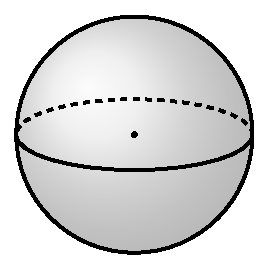
\includegraphics[width=.3\textwidth]{figures/sphere/Sphere1.pdf}
	$$\mathbb{P}^1= \{ \infty \} \sqcup \mathbb{A}^1$$
\end{minipage}
\begin{minipage}[b]{.45\textwidth}
\centering
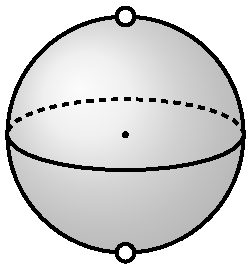
\includegraphics[width=.3\textwidth]{figures/sphere/Sphere3.pdf}
$$\mathbb{P}^1 \smallsetminus \{0,\infty \} \text{ has no affine paving}$$
\end{minipage}
\end{figure}

\end{frame}

\begin{frame}[fragile,t]{Quiver and quiver representation}
\begin{short}
\begin{center}
\begin{tabular}{@{\extracolsep{4mm}}ccc}
$$\begin{tikzcd}[ampersand replacement=\&, column sep=4mm]
	\scriptstyle\bullet \& \scriptstyle\bullet \& \scriptstyle\bullet \& \scriptstyle\bullet
	\arrow[from=1-1, to=1-2]
	\arrow[from=1-3, to=1-2]
	\arrow[from=1-4, to=1-3]
\end{tikzcd}$$ & $$\begin{tikzcd}[ampersand replacement=\&]
 	\scriptstyle\bullet \arrow[out=-30,in=30,loop,looseness=8]
 \end{tikzcd}$$ & $$\begin{tikzcd}[ampersand replacement=\&, column sep=8mm]
 	\scriptstyle\bullet \& \scriptstyle\bullet
 	\arrow[curve={height=-6pt}, from=1-1, to=1-2]
 	\arrow[curve={height=6pt}, from=1-1, to=1-2]
 \end{tikzcd}$$ 
\end{tabular}
\end{center}
\end{short}

\only<1>{Quiver is a graph. It has some vertices $\&$ arrows.\\
In this talk, all the quivers are finite and connected.
}

\only<2>{
We focus on the Dynkin quiver.\\
That means, the graph of the Dynkin diagrams in the ADE series.
}

\only<2>{
\begin{short}
\tikzcdset{arrow style=tikz,
           diagrams={>=Classical TikZ Rightarrow,shorten <=-2pt,shorten >=-2pt,}
           }
\begin{center}
\begin{tabular}{@{\extracolsep{3mm}}ccc}
$$\begin{tikzcd}[ampersand replacement=\&, sep=2mm]
	\& \scriptstyle\bullet \\
	\scriptstyle\bullet \& \scriptstyle\bullet \& \scriptstyle\bullet \& \scriptstyle\bullet
	\arrow[from=2-1, to=2-2]
	\arrow[from=1-2, to=2-2]
	\arrow[from=2-2, to=2-3]
	\arrow[from=2-4, to=2-3]
\end{tikzcd}$$
& $$\begin{tikzcd}[ampersand replacement=\&, sep=2mm]
	\&\& \scriptstyle\bullet \\
	\scriptstyle\bullet \& \scriptstyle\bullet \& \scriptstyle\bullet \& \scriptstyle\bullet \& \scriptstyle\bullet
	\arrow[from=2-3, to=2-4]
	\arrow[from=2-2, to=2-1]
	\arrow[from=1-3, to=2-3]
	\arrow[from=2-3, to=2-2]
	\arrow[from=2-4, to=2-5]
\end{tikzcd}$$
 & $$\begin{tikzcd}[ampersand replacement=\&, sep=2mm]
 \&\&\&\\
 	\scriptstyle\bullet \&[6mm] \scriptstyle\bullet \& \scriptstyle\bullet \& \scriptstyle\bullet
 	\arrow[from=2-2, to=2-3]
 	\arrow[out=-20,in=200, from=2-1, to=2-2]
 	\arrow[from=2-4, to=2-3]
 	\arrow[out=20,in=160, from=2-1, to=2-2]
 \end{tikzcd}$$
  \\[2mm]
 $D_5$ & $E_6$ & $B_4$
\end{tabular}
\end{center}
\end{short}

%https://tex.stackexchange.com/questions/89588/positioning-relative-to-page-in-tikz
	\begin{tikzpicture}[remember picture,overlay]
	\coordinate (center) at ([xshift=36mm, yshift=-13mm]current page.center);
	  % Draw a cross at the center of the page
	  \draw[red, line width=3pt] (center) -- ++(-1,0.5) -- ++(2,-1);
	  \draw[red, line width=3pt] (center) -- ++(1,0.5) -- ++(-2,-1);
	\end{tikzpicture}
}
\end{frame}
% https://q.uiver.app/?q=WzAsNSxbMCwxLCJcXGJ1bGxldCJdLFsxLDEsIlxcYnVsbGV0Il0sWzEsMCwiXFxidWxsZXQiXSxbMiwxLCJcXGJ1bGxldCJdLFszLDEsIlxcYnVsbGV0Il0sWzAsMV0sWzIsMV0sWzEsM10sWzQsM11d
% https://q.uiver.app/?q=WzAsNSxbMCwxLCJWXzEiXSxbMSwxLCJWXzIiXSxbMSwwLCJWXzUiXSxbMiwxLCJWXzMiXSxbMywxLCJWXzQiXSxbMCwxLCJcXGFscGhhIl0sWzIsMSwiXFxkZWx0YSJdLFsxLDMsIlxcYmV0YSJdLFs0LDMsIlxcZ2FtbWEiLDJdXQ==
% https://q.uiver.app/?q=WzAsNSxbMCwxLCJcXG1hdGhiYntDfV57Mn0iXSxbMSwxLCJcXG1hdGhiYntDfV57Mn0iXSxbMSwwLCIwIl0sWzIsMSwiXFxtYXRoYmJ7Q31eezJ9Il0sWzMsMSwiXFxtYXRoYmJ7Q30iXSxbMCwxLCJcXElkIl0sWzIsMV0sWzEsMywiXFxJZCJdLFs0LDMsIihcXCEgXFxiZWdpbntzbWFsbG1hdHJpeH0gXFxzY3JpcHRzdHlsZSAxICYgIFxcc2NyaXB0c3R5bGUgMCAgXFxlbmR7c21hbGxtYXRyaXh9XFwhKSIsMl1d
\begin{frame}[fragile]{Quiver representation}
\begin{short}
\begin{center}
\begin{tabular}{cc}
$$
\begin{tikzcd}[ampersand replacement=\&, sep={between origins, 11mm}]
	\& \bullet \& \& \\
	\bullet \& \bullet \& \bullet \& \bullet
	\arrow[from=2-1, to=2-2]
	\arrow[from=1-2, to=2-2]
	\arrow[from=2-2, to=2-3]
	\arrow[from=2-4, to=2-3]
\end{tikzcd}
$$
& 
\only<1>{$$\begin{tikzcd}[ampersand replacement=\&, sep={between origins, 11mm}]
	\& {V_5}  \& \& \\
	{V_1} \& {V_2} \& {V_3} \& {V_4}
	\arrow["\alpha", from=2-1, to=2-2]
	\arrow["\delta", from=1-2, to=2-2]
	\arrow["\beta", from=2-2, to=2-3]
	\arrow["\gamma"', from=2-4, to=2-3]
\end{tikzcd}$$}
\only<2-3>{$$\begin{tikzcd}[ampersand replacement=\&, sep={between origins, 11mm},>=Classical TikZ Rightarrow,shorten <=-3pt,shorten >=-3pt]
	\& 0 \& \& \\
	{\mathbb{C}^{2}} \& {\mathbb{C}^{2}} \& {\mathbb{C}^{2}} \& {\mathbb{C}}
	\arrow["\scriptscriptstyle\Id", from=2-1, to=2-2]
	\arrow[from=1-2, to=2-2]
	\arrow["\scriptscriptstyle\Id", from=2-2, to=2-3]
	\arrow["{(\! \begin{smallmatrix} \scriptscriptstyle 1 &  \scriptscriptstyle 0  \end{smallmatrix}\!)}"', from=2-4, to=2-3]
\end{tikzcd}$$}
  \\[10mm]
 $Q$ & $V \in \rep(Q)$ \\[5mm]
 \visible<3->{Dimension vector:} &  \visible<3->{$\dimv V= \substack{0\phantom{0}\\2221}$}
 \\[0mm]
\end{tabular}
\end{center}
\end{short}

%\only<4>{
%\begin{eg}
%When $Q= \bullet$, $\rep(Q)= \Vect_{\mathbb{C}}$.
%\end{eg}
%}
\end{frame}


%https://tex.stackexchange.com/questions/436284/how-to-adjust-parenthesis-thickness-without-changing-the-font
%https://tex.stackexchange.com/questions/207056/wrong-too-much-vertical-space-above-vdots-in-small-matrix
\begin{frame}[fragile]{Partial flag variety}
\begin{definition}
Fix a quiver $Q$ and $M \in \rep(Q)$,
\begin{equation*}
\begin{aligned}
\Flag_{d}(M)\colon=\;& \left\{ F\colon 0 \subseteq N_1 \subseteq \cdots\subseteq N_d \subseteq M  \right\} \\ 
\Flag_{\ftdimvec{f}}(M)\colon=\;&\left\{ F\colon 0 \subseteq N_1 \subseteq \cdots\subseteq N_d \subseteq M \;\middle|\;\rule{0mm}{3.4mm} \dimv N_i =\ftdimvec{f}_i \right\}
\end{aligned}
\end{equation*}
\end{definition}
\visible<2>{
\begin{eg}
$Q= \bullet$, $M=\mathbb{C}^n$, \\[-4mm]
%$\ftdimvec{f}:=\scalemath{0.7}
%{\left(
%\begin{smallmatrix}
%\scriptsize n \\ \vphantom{\int\limits^x}\smash{\vdots} \\ 1
%\end{smallmatrix}
%\right)}$
\begin{equation*}
\begin{aligned}
%\Flag_{d}(\mathbb{C}^n)=\;& \left\{ F\colon 0 \subseteq N_1 \subseteq \cdots\subseteq N_d \subseteq \mathbb{C}^n  \right\}\hspace{-10mm}& \\ 
\Flag_{1}(\mathbb{C}^n)=\;& \left\{ F\colon 0 \subseteq N_1  \subseteq \mathbb{C}^n  \right\} &= \bigsqcup_{k=0}^{n} \Gr (n,k) \\[-3mm]
%\Flag_{\ftdimvec{f}}(\mathbb{C}^n)=\;&\text{ complete flags of $\mathbb{C}^n$} & \\
\Flag_{(k)}(\mathbb{C}^n)=\;& \Gr (n,k) &\\
\end{aligned}
\end{equation*}
\end{eg}
}

\end{frame}


\begin{frame}[fragile]{Statement}
\begin{theorem}
For a Dynkin quiver $Q$ and $M \in \rep(Q)$, 
$$\Flag_{d}(M) \text{ has an affine paving.}$$
\end{theorem}

\end{frame}


%%%%%%%%%%%%%%%%%%%%%%%%%%%%%%%%%%%%
\section{Case study}
\begin{frame}{Process}
\tableofcontents[currentsection,hideallsubsections]
\end{frame}


\begin{frame}[fragile]{Task 1. $Q= \bullet$, $M=\mathbb{C}^n$}
\visible<2->{
In this case,
% https://q.uiver.app/?q=WzAsOSxbMCwwLCJcXEdMX24oXFxtYXRoYmJ7Q30pIFxcLFxccm90YXRlYm94W29yaWdpbj1jXXsyNzB9eyRcXGNpcmNsZWFycm93cmlnaHQkfVxcOyBcXG1hdGhiYntDfV5uIl0sWzMsMCwiXFxHTF9uKFxcbWF0aGJie0N9KSAiXSxbMywxLCJCICJdLFsyLDFdLFs0LDEsIlxccm90YXRlYm94W29yaWdpbj1jXXsyNzB9eyRcXGNpcmNsZWFycm93cmlnaHQkfVxcOyBcXEZsYWdfe2R9KFxcbWF0aGJie0N9Xm4pIl0sWzQsMCwiXFxyb3RhdGVib3hbb3JpZ2luPWNdezI3MH17JFxcY2lyY2xlYXJyb3dyaWdodCR9XFw7IFxcRmxhZ197ZH0oXFxtYXRoYmJ7Q31ebikiXSxbMSwwXSxbMiwwXSxbMSwxXSxbNiw3LCIiLDAseyJzdHlsZSI6eyJib2R5Ijp7Im5hbWUiOiJzcXVpZ2dseSJ9fX1dLFs4LDMsIiIsMCx7InN0eWxlIjp7ImJvZHkiOnsibmFtZSI6InNxdWlnZ2x5In19fV1d
\[\begin{tikzcd}[row sep=0mm, column sep=0mm, ampersand replacement=\&,]
{\GL_n(\mathbb{C}) \,\rotatebox[origin=c]{270}{$\circlearrowright$}\; \mathbb{C}^n} \& {} \&[20mm] {} \& {\GL_n(\mathbb{C}) } \&[-3mm] {\rotatebox[origin=c]{270}{$\circlearrowright$}\; \Flag_{d}(\mathbb{C}^n)} \\
\& {} \& {} \& {B } \& {\rotatebox[origin=c]{270}{$\circlearrowright$}\; \Flag_{d}(\mathbb{C}^n)}
\arrow[squiggly, from=1-2, to=1-3]
\arrow[squiggly, from=2-2, to=2-3]
\end{tikzcd}\]

$\Flag_{d}(\mathbb{C}^n)$ has an affine paving given by Schubert cells (i.e., $B$-orbits).
}

\visible<3>{
\begin{block}{Note}
When $Q= \bullet \longrightarrow \bullet$, $\Flag_{\dimvec{f}}(M)$ have no natural group actions.
\end{block}
}


\end{frame}



\begin{frame}[fragile]{Task 2a. $Q= {\textstyle\bullet \rightarrow \bullet}$, $M=\left[\mathbb{C}^2 \stackrel{\scriptstyle 0}{\rightarrow}\mathbb{C}^2\right]$, $d=1$}

\visible<2->{
\begin{equation*}
\begin{aligned}
\ftdimvec{f}=(1,0):\;& \quad\quad \Flag_{\ftdimvec{f}}(M) = \mathbb{P}^1 \\
\ftdimvec{f}=(0,0):\;&  \quad\quad\Flag_{\ftdimvec{f}}(M) = \pt \\
  \ftdimvec{f}=(1,1):\;& \quad\quad \Flag_{\ftdimvec{f}}(M) = \mathbb{P}^1 \times \mathbb{P}^1 \\
\end{aligned}
\end{equation*}
$\,$\\[5mm]
}

\visible<3->{
In this case, 
$$\Flag_{(a,b)}(M) \cong \Flag_{(a)}(\mathbb{C}^2) \times \Flag_{(b)}(\mathbb{C}^2) $$
has an affine paving.
}



\end{frame}

\begin{frame}[fragile]{Task 2b. $Q= {\textstyle\bullet \rightarrow \bullet}$, $M=\left[\mathbb{C}^2 \stackrel{\scriptstyle\Id}{\rightarrow}\mathbb{C}^2\right]$, $d=1$}

\visible<2->{
\begin{equation*}
\begin{aligned}
\ftdimvec{f}=(1,0):\;& \quad\quad \Flag_{\ftdimvec{f}}(M) = \varnothing \\
\ftdimvec{f}=(0,0):\;&  \quad\quad\Flag_{\ftdimvec{f}}(M) = \pt \\
\ftdimvec{f}=(1,1):\;& \quad\quad \Flag_{\ftdimvec{f}}(M) = \mathbb{P}^1 \\
\ftdimvec{f}=(0,1):\;& \quad\quad \Flag_{\ftdimvec{f}}(M) = \mathbb{P}^1 \\
\end{aligned}
\end{equation*}
$\,$\\[5mm]
}

\visible<3->{
In this case, 
$$\Flag_{(a,b)}(M) \cong \Flag_{\left( \substack{b\\a} \right)}(\mathbb{C}^2)$$
has an affine paving.
}



\end{frame}

\begin{frame}[fragile]{Task 2c. $Q= {\textstyle\bullet \rightarrow \bullet}$, $M=\left[\mathbb{C}^2 \stackrel{
\left(\!
\begin{smallmatrix}
\scriptscriptstyle 1 &  \scriptscriptstyle 0 \\[-0.6mm] \scriptscriptstyle 0 & \scriptscriptstyle 0
\end{smallmatrix}\!\right)}{\longrightarrow}\mathbb{C}^2\right]$, $d=1$}

\visible<2->{
\begin{equation*}
\begin{aligned}
\ftdimvec{f}=(1,0):\;& \quad\quad \Flag_{\ftdimvec{f}}(M) = \pt \\
\ftdimvec{f}=(0,0):\;&  \quad\quad\Flag_{\ftdimvec{f}}(M) = \pt \\
  \ftdimvec{f}=(1,1):\;& \quad\quad \Flag_{\ftdimvec{f}}(M) = \mathbb{P}^1 \vee \mathbb{P}^1 \\
  \ftdimvec{f}=(0,1):\;& \quad\quad \ldots \\
\end{aligned}
\end{equation*}
$\,$\\[5mm]
}

\visible<3->{
To construct affine pavings systematically, we need to construct an uniform method.
}
\end{frame}

\begin{frame}[fragile]{Task 2c. $Q= {\textstyle\bullet \rightarrow \bullet}$, $M=\left[\mathbb{C}^2 \stackrel{
\left(\!
\begin{smallmatrix}
\scriptscriptstyle 1 &  \scriptscriptstyle 0 \\[-0.6mm] \scriptscriptstyle 0 & \scriptscriptstyle 0
\end{smallmatrix}\!\right)}{\longrightarrow}\mathbb{C}^2\right]$, $d=1$}

\begin{block}{First try}
Let $X= \left[ 0 
\stackrel{\phantom{
(\!
\begin{smallmatrix}
\scriptstyle 1 &  \scriptstyle 0 
\end{smallmatrix}\!)}}{\longrightarrow}
 \mathbb{C} \right]$, $S= \left[ \mathbb{C}^{2} \stackrel{
(\!
\begin{smallmatrix}
\scriptstyle 1 &  \scriptstyle 0 
\end{smallmatrix}\!)}{\longrightarrow} \mathbb{C} \right]$, then $M=X \oplus S$,\\ and the short exact sequence 
% https://q.uiver.app/?q=WzAsNSxbMSwwLCJYIl0sWzIsMCwiTSJdLFszLDAsIlMiXSxbNCwwLCIwIl0sWzAsMCwiMCJdLFs0LDBdLFswLDEsIlxcaW90YSJdLFsxLDIsIlxccGkiXSxbMiwzXV0=
\[\begin{tikzcd}
0 & X & M & S & 0
\arrow[from=1-1, to=1-2]
\arrow["\iota", from=1-2, to=1-3]
\arrow["\pi", from=1-3, to=1-4]
\arrow[from=1-4, to=1-5]
\end{tikzcd}\]
induces
\begin{equation*}
\begin{aligned}
\Psi: \Flag_{d}(M) \longrightarrow\;& \Flag_{d}(X) \times \Flag_{d}(S) \\ 
F\hspace{5mm} \longmapsto\;& \hspace{5mm}\left( \iota^{-1}(F), \pi(F) \right)
\end{aligned}
\end{equation*}
\end{block}

\end{frame}

\begin{frame}[fragile]{Idea of affine pavings}
Find a nice short exact sequence 
$$0\longrightarrow X \stackrel{\iota}{\longrightarrow} M \stackrel{\pi}{\longrightarrow} S \longrightarrow 0$$
which induces a nice morphism
\begin{equation*}
\begin{aligned}
\Psi: \Flag_{d}(M) \longrightarrow\;& \Flag_{d}(X) \times \Flag_{d}(S) \\ 
F\hspace{5mm} \longmapsto\;& \hspace{5mm}\left( \iota^{-1}(F), \pi(F) \right)
\end{aligned}
\end{equation*}
We construct the affine paving of $\Flag_{d}(M)$ from the affine paving of $\Flag_{d}(X)$ and $\Flag_{d}(S)$. Then, we use mathematical induction.
\end{frame}

\begin{frame}[fragile]{Example.  $Q= \bullet$, $M=\mathbb{C}^2$}

% https://q.uiver.app/?q=WzAsNSxbMSwwLCJcXG1hdGhiYntDfSJdLFsyLDAsIlxcbWF0aGJie0N9XjIiXSxbMywwLCJcXG1hdGhiYntDfSJdLFs0LDAsIjAiXSxbMCwwLCIwIl0sWzQsMF0sWzAsMSwiXFxpb3RhIl0sWzEsMiwiXFxwaSJdLFsyLDNdXQ==
\[\begin{tikzcd}[ampersand replacement=\&]
0 \& {\mathbb{C}} \& {\mathbb{C}^2} \& {\mathbb{C}} \& 0
\arrow[from=1-1, to=1-2]
\arrow["\iota", from=1-2, to=1-3]
\arrow["\pi", from=1-3, to=1-4]
\arrow[from=1-4, to=1-5]
\end{tikzcd}\]

\visible<2->{
% https://q.uiver.app/?q=WzAsMTQsWzEsMCwiXFxGbGFnX3sxfShcXG1hdGhiYntDfV4yKSJdLFsyLDAsIlxcRmxhZ197MX0oXFxtYXRoYmJ7Q30pIFxcdGltZXMgXFxGbGFnX3sxfShcXG1hdGhiYntDfSkiXSxbMywwXSxbNCwwXSxbMSwxLCJcXEZsYWdicmF7MX0oXFxtYXRoYmJ7Q30pIl0sWzIsMSwiXFxGbGFnYnJhezF9KFxcbWF0aGJie0N9KSBcXHRpbWVzIFxcRmxhZ2JyYXswfShcXG1hdGhiYntDfSkiXSxbNCwxLCJcXEZsYWdicmF7MH0oXFxtYXRoYmJ7Q30pIFxcdGltZXMgXFxGbGFnYnJhezF9KFxcbWF0aGJie0N9KSJdLFszLDEsIlxcYmlnc3FjdXAiXSxbMSwyLCJcXG1hdGhiYntQfV4xIl0sWzIsMiwiXFx7KlxcfSJdLFs0LDIsIlxceypcXH0iXSxbMywyLCJcXGJpZ3NxY3VwIl0sWzAsMSwiXFxQc2lfeygxKX06Il0sWzAsMCwiXFxQc2lfMToiXSxbNCw1XSxbMCwxXSxbOCw5XV0=
\adjustbox{scale=0.88,center}{
\begin{tikzcd}[row sep=tiny, column sep={-2mm}, scale=0.6, ampersand replacement=\&]
{\Psi_1:} \& {\Flag_{1}(\mathbb{C}^2)} \&[10mm] {\Flag_{1}(\mathbb{C}) \times \Flag_{1}(\mathbb{C})} \& {} \& {} \\
{\Psi_{(1)}:} \& {\Flagbra{1}(\mathbb{C}^2)} \& {\Flagbra{1}(\mathbb{C}) \times \Flagbra{0}(\mathbb{C})} \& \bigsqcup \& {\Flagbra{0}(\mathbb{C}) \times \Flagbra{1}(\mathbb{C})} \\[-3mm]
\& {\mathbb{P}^1} \& {\pt} \& \bigsqcup \& {\pt}
\arrow[shorten >=3mm, from=1-2, to=1-3]
\arrow[shorten >=0mm, from=2-2, to=2-3]
\arrow[shorten <=7mm, shorten >=17mm, from=3-2, to=3-3]
\end{tikzcd}
}
}

%\visible<3->{
%\begin{block}{Question}
%How does $\Psi_{(1)}$ give an affine paving of $\Flagbra{1}(\mathbb{C}^2)$?
%\end{block}
%}
% https://q.uiver.app/?q=WzAsMyxbMSwxLCJcXHB0IFxcc3FjdXAgXFxwdCJdLFsxLDAsIlxce1xcaW5mdHlcXH0gXFxzcWN1cCBcXG1hdGhiYntDfSJdLFswLDAsIlxcbWF0aGJie1B9XjEiXSxbMiwxLCI9IiwxLHsic3R5bGUiOnsiYm9keSI6eyJuYW1lIjoibm9uZSJ9LCJoZWFkIjp7Im5hbWUiOiJub25lIn19fV0sWzEsMCwiXFxQc2lfeygxKX0iXV0=
\vspace{-5mm}
\visible<3->{
\[\begin{tikzcd}[column sep={0mm},row sep={10mm}, ampersand replacement=\&]
{\mathbb{P}^1} \& {\{\infty\} \sqcup \,\mathbb{C}} \phantom{\{\}}\\
\& {\pt \sqcup \pt}
\arrow["{=}"{description}, draw=none, from=1-1, to=1-2]
\arrow["{\Psi_{(1)}}", from=1-2, to=2-2]
\end{tikzcd}\]
}
\end{frame}

\begin{frame}[fragile]{Example.  $Q= \bullet$, $M=\mathbb{C}^8=\bigoplus_{i=1}^{8} \mathbb{C}v_i$}

% https://q.uiver.app/?q=WzAsNSxbMSwwLCJcXG1hdGhiYntDfSJdLFsyLDAsIlxcbWF0aGJie0N9XjIiXSxbMywwLCJcXG1hdGhiYntDfSJdLFs0LDAsIjAiXSxbMCwwLCIwIl0sWzQsMF0sWzAsMSwiXFxpb3RhIl0sWzEsMiwiXFxwaSJdLFsyLDNdXQ==
\[\begin{tikzcd}[ampersand replacement=\&]
0 \& {\mathbb{C}^3} \& {\mathbb{C}^8} \& {\mathbb{C}^5} \& 0
\arrow[from=1-1, to=1-2]
\arrow["\iota", from=1-2, to=1-3]
\arrow["\pi", from=1-3, to=1-4]
\arrow[from=1-4, to=1-5]
\end{tikzcd}\]
\vspace{-2mm}
% https://q.uiver.app/?q=WzAsMixbMSwwLCJcXEZsYWdicmF7MX0oXFxtYXRoYmJ7Q31eMykgXFx0aW1lcyBcXEZsYWdicmF7Mn0oXFxtYXRoYmJ7Q31eNSkiXSxbMCwwLCJcXEZsYWdicmF7M30oXFxtYXRoYmJ7Q31eOCkiXSxbMSwwLCIiLDAseyJzdHlsZSI6eyJib2R5Ijp7Im5hbWUiOiJkYXNoZWQifX19XV0=
\[\begin{tikzcd}[ampersand replacement=\&]
\Psi: {\Flagbra{3}(\mathbb{C}^8)} \& {\Flagbra{1}(\mathbb{C}^3) \times \Flagbra{2}(\mathbb{C}^5) \;\bigsqcup\; \cdots}
\arrow[from=1-1, to=1-2]
\end{tikzcd}\]
\vspace{-10mm}

\begin{equation*}
\begin{aligned}
\Psi^{-1}\!\left(\!  \left< v_1 \right>\!,\!\rule{0mm}{3.7mm} \left< v_4,\!v_5 \right> \! \right) =\;&  \left\{\left< v_1, v_4\!+\!av_2\! +\!bv_3 ,v_5\! +\!cv_2\! +\!dv_3 \right>\rule{0mm}{3.7mm}  \middle|\;  a,b,c,d \in \mathbb{C}  \right\} \\ 
\cong\;& \;\;\mathbb{C}^4
\end{aligned}
\end{equation*}
\visible<2->{
\begin{short}
$\Psi$ is a Zarisky-locally trivial affine bundle of rank $2 \cdot (3-1)=4$.
\end{short}
}
\end{frame}


\begin{frame}[fragile]
\noindent Consider the short exact sequence of representations
\vspace{-3mm}
\[\begin{tikzcd}
\eta: 0 & {X} & {Y} & {S} & 0
\arrow[from=1-1, to=1-2]
\arrow["\iota", from=1-2, to=1-3]
\arrow["\pi", from=1-3, to=1-4]
\arrow[from=1-4, to=1-5]
\end{tikzcd}\]

\vspace{-4mm}
\noindent which induce maps
\vspace{-4mm}
% https://q.uiver.app/?q=WzAsNixbMSwwLCIgXFxGbGFnX2QoWSkiXSxbMiwwLCJcXEZsYWdfZChYKSBcXHRpbWVzIFxcRmxhZ19kKFMpIl0sWzEsMSwiXFxGbGFnKFkpX3tcXGZ0ZGltdmVje2Z9LFxcZnRkaW12ZWN7Z319Il0sWzIsMSwiXFxGbGFnX3tcXGZ0ZGltdmVje2Z9fShYKSBcXHRpbWVzIFxcRmxhZ197XFxmdGRpbXZlY3tnfX0oUykiXSxbMCwwLCJcXFBzaToiXSxbMCwxLCJcXFBzaV97XFxmdGRpbXZlY3tmfSxcXGZ0ZGltdmVje2d9fTogIl0sWzIsM10sWzAsMV0sWzIsMCwiXFxzdWJzZXQiLDEseyJzdHlsZSI6eyJib2R5Ijp7Im5hbWUiOiJub25lIn0sImhlYWQiOnsibmFtZSI6Im5vbmUifX19XSxbMywxLCJcXHN1YnNldCIsMSx7InN0eWxlIjp7ImJvZHkiOnsibmFtZSI6Im5vbmUifSwiaGVhZCI6eyJuYW1lIjoibm9uZSJ9fX1dXQ==
\[\begin{tikzcd}[row sep={1mm}]
	{\phantom{f,g}\Psi:} &[-10mm] { \Flag_d(Y)} & {\Flag_d(X) \times \Flag_d(S)} \\
	{\Psi_{\ftdimvec{f},\ftdimvec{g}}: } & {\Flag(Y)_{\ftdimvec{f},\ftdimvec{g}}} & {\Flag_{\ftdimvec{f}}(X) \times \Flag_{\ftdimvec{g}}(S)}
	\arrow[from=2-2, to=2-3]
	\arrow[from=1-2, to=1-3]
	\arrow["\subset"{description}, sloped, draw=none, from=2-2, to=1-2]
	\arrow["\subset"{description}, sloped, draw=none, from=2-3, to=1-3]
\end{tikzcd}\]
\vspace{-6mm}
\visible<2->{
\begin{block}{Theorem A}
When $\eta$ splits, then $\Psi$ is surjective. \\
Moreover, if $\Ext^1(S,X)=0$, then
\vspace{-2mm}
\begin{center}
$\Psi_{\ftdimvec{f},\ftdimvec{g}}$ is a Zarisky-locally trivial affine bundle.
\end{center}
\end{block}
}

\visible<3->{
\noindent By this theorem, 
\vspace{-3mm}
\begin{center}
\fbox{
$\Flag_{d}(Y)$ has an affine paving $\Longleftarrow$ $\Flag_{d}(X)$, $\Flag_{d}(S)$ have.}
\end{center}
}
\end{frame}



\begin{frame}[fragile]{\textcolor{red}{Warming}}
$\eta$ splits and $\Ext^1(S,X)=0$ are necessary for Theorem A.

\visible<2->{
\begin{eg}
Consider the quiver $Q: {\textstyle\bullet \rightarrow \bullet \leftarrow \bullet}$ and the short exact sequence 
% https://q.uiver.app/?q=WzAsNSxbMSwwLCJcXGxlZnRbICBcXG1hdGhiYntDfWVfMSBcXHJpZ2h0YXJyb3cgXFxtYXRoYmJ7Q31eMiBcXGxlZnRhcnJvdyBcXG1hdGhiYntDfWVfMiBcXHJpZ2h0XSJdLFsyLDAsIlxcbGVmdFsgIFxcbWF0aGJie0N9XjIgXFxzdGFja3JlbHtcXHNjcmlwdHNjcmlwdHN0eWxlXFxJZH17XFxyaWdodGFycm93fSBcXG1hdGhiYntDfV4yIFxcc3RhY2tyZWx7XFxzY3JpcHRzY3JpcHRzdHlsZVxcSWR9e1xcbGVmdGFycm93fSBcXG1hdGhiYntDfV4yIFxccmlnaHRdIl0sWzMsMCwiXFxsZWZ0WyAgXFxtYXRoYmJ7Q31lXzIgXFxyaWdodGFycm93IDAgXFxsZWZ0YXJyb3cgXFxtYXRoYmJ7Q31lXzEgXFxyaWdodF0iXSxbNCwwLCIwIl0sWzAsMCwiMCJdLFswLDFdLFsxLDJdLFsyLDNdLFs0LDBdXQ==
\adjustbox{scale=0.77,center}{
\begin{tikzcd}[row sep={14mm}, ampersand replacement=\&]
	0 \&[-3mm] {\left[  \mathbb{C}e_1 \stackrel{\scriptscriptstyle\phantom{\Id}}{\rightarrow} \mathbb{C}^2 \leftarrow \mathbb{C}e_2 \right]} \& {\left[  \mathbb{C}^2 \stackrel{\scriptscriptstyle\Id}{\rightarrow} \mathbb{C}^2 \stackrel{\scriptscriptstyle\Id}{\leftarrow} \mathbb{C}^2 \right]} \& {\left[  \mathbb{C}e_2 \stackrel{\scriptscriptstyle\phantom{\Id}}{\rightarrow} 0 \leftarrow \mathbb{C}e_1 \right]} \&[-3mm] 0
	\arrow[from=1-2, to=1-3]
	\arrow[from=1-3, to=1-4]
	\arrow[from=1-4, to=1-5]
	\arrow[from=1-1, to=1-2]
\end{tikzcd}
}
\vspace{0mm}

\visible<3->{
we get
\vspace{-3mm}
$$\Img \Psi_{(0,1,0),(1,0,1)} \cong \left(  \mathbb{P}^1 \smallsetminus \{0, \infty \}\right) \times \pt  \cong \mathbb{C}^*,$$
\vspace{-7mm}

so $\Psi$ is not surjective.\\[3mm]
}
\visible<4->{
In this way, we get a bad stratification
\vspace{-3mm}
$$\Flag_{(1,1,1)}(Y) \cong \mathbb{P}^1 = \{0\} \sqcup \{\infty\} \sqcup \mathbb{C}^{*}.$$
\vspace{-3mm}
}
\end{eg}
}

\end{frame}

\begin{frame}[fragile,t]{Task 3. $Q= {\scriptstyle
% https://q.uiver.app/?q=WzAsNCxbMSwwLCJcXGJ1bGxldCJdLFsxLDEsIlxcYnVsbGV0Il0sWzAsMSwiXFxidWxsZXQiXSxbMiwxLCJcXGJ1bGxldCJdLFswLDFdLFsyLDFdLFszLDFdXQ==
\adjustbox{scale=0.7}{
\begin{tikzcd}[sep={between origins, 10mm}, ampersand replacement=\&]
	\& \scriptstyle\bullet \&\\
	\scriptstyle\bullet \& \scriptstyle\bullet \& \scriptstyle\bullet\\[-6mm]
	\arrow[from=1-2, to=2-2]
	\arrow[from=2-1, to=2-2]
	\arrow[from=2-3, to=2-2]
\end{tikzcd}
}
}$, $M=\substack{1\\121} \oplus \substack{1\\111} \oplus \substack{1\\111}$}

We use following short exact sequences
% https://q.uiver.app/?q=WzAsMTAsWzIsMSwiXFxzdWJzdGFja3sxXFxcXDExMX0gXFxvcGx1cyBcXHN1YnN0YWNrezFcXFxcMTExfSJdLFszLDEsIlxcc3Vic3RhY2t7MVxcXFwxMTF9Il0sWzEsMSwiXFxzdWJzdGFja3sxXFxcXDExMX0iXSxbMywwLCJcXHN1YnN0YWNrezFcXFxcMTIxfSJdLFsxLDAsIlxcc3Vic3RhY2t7MVxcXFwxMTF9IFxcb3BsdXMgXFxzdWJzdGFja3sxXFxcXDExMX0iXSxbMiwwLCJNIl0sWzAsMCwiMCJdLFs0LDAsIjAiXSxbMCwxLCIwIl0sWzQsMSwiMCJdLFs2LDRdLFs0LDVdLFs1LDNdLFszLDddLFs4LDJdLFsyLDBdLFswLDFdLFsxLDldXQ==
\[\begin{tikzcd}[row sep=tiny]
	0 & {\substack{1\\111} \oplus \substack{1\\111}} & M & {\substack{1\\121}} & 0 \\
	0 & {\substack{1\\111}} & {\substack{1\\111} \oplus \substack{1\\111}} & {\substack{1\\111}} & 0
	\arrow[from=1-1, to=1-2]
	\arrow[from=1-2, to=1-3]
	\arrow[from=1-3, to=1-4]
	\arrow[from=1-4, to=1-5]
	\arrow[from=2-1, to=2-2]
	\arrow[from=2-2, to=2-3]
	\arrow[from=2-3, to=2-4]
	\arrow[from=2-4, to=2-5]
\end{tikzcd}\]

to reduced the problem to indecomposable representations.

\only<2->{
\hrulefill
}

%This paragraph should be omitted after the first show.
\only<2-3>{Notice that we use the result
$$\Ext^1 \!\left(\rule{0mm}{3.4mm} \substack{1\\121}, \substack{1\\111}  \right)=0, \qquad \Ext^1 \!\left(\rule{0mm}{3.4mm} \substack{1\\111}, \substack{1\\111}  \right)=0.$$}

\only<3>{We can't put $\substack{1\\121}$ on the left, since
$$\Ext^1 \!\left(\rule{0mm}{3.4mm} \substack{1\\111}, \substack{1\\121}  \right) \cong \mathbb{C}  \neq 0.$$}

%This paragraph should be shown later.
\only<4->{$\Flag_{d} \left(\substack{1\\111} \right)$ has an affine paving: obvious.

$\Flag_{d} \left(\substack{1\\121} \right)$ has an affine paving: it is $\mathbb{P}^1$, $\pt$ or empty.}

\only<5>{
\hrulefill

Need: more informations of indecomposable representations!
}

\end{frame}


%%%%%%%%%%%%%%%%%%%%%%%%%%%%%%%%%%%%%%%%%%%%%
\section{Auslander--Reiten theory}
\begin{frame}{Process}
\tableofcontents[currentsection,hideallsubsections]
\end{frame}

%initial picture
\begin{frame}[fragile,t]{Auslander--Reiten quiver: $D_4 \qquad$% https://q.uiver.app/?q=WzAsNCxbMCwxLCIxIl0sWzEsMSwiMiJdLFsyLDEsIjMiXSxbMSwwLCI0Il0sWzAsMV0sWzIsMV0sWzMsMV1d
\tikzcdset{arrow style=tikz,
           diagrams={>=Classical TikZ Rightarrow,shorten <=-3pt,shorten >=-3pt,}
           }
\begin{tikzcd}[sep={1mm},font = \footnotesize, ampersand replacement=\&]
\& 4 \\
2 \& 1 \& 3
\arrow[from=2-1, to=2-2]
\arrow[from=2-3, to=2-2]
\arrow[from=1-2, to=2-2]
\end{tikzcd}}

\begin{short}
\vspace{-5mm}
%\[\begin{tikzcd}[column sep={2cm,between origins},row sep={13mm,between origins}]
% https://q.uiver.app/?q=WzAsMTYsWzIsMSwiXFxzdWJzdGFja3swXFxcXDAxMH0iXSxbMywwLCJcXHN1YnN0YWNrezBcXFxcMTEwfSJdLFszLDMsIlxcc3Vic3RhY2t7MFxcXFwwMTF9Il0sWzMsMiwiXFxzdWJzdGFja3sxXFxcXDAxMH0iXSxbNCwxLCJcXHN1YnN0YWNrezFcXFxcMTIxfSJdLFs1LDAsIlxcc3Vic3RhY2t7MVxcXFwwMTF9Il0sWzUsMywiXFxzdWJzdGFja3sxXFxcXDExMH0iXSxbNSwyLCJcXHN1YnN0YWNrezBcXFxcMTExfSJdLFs3LDAsIlxcc3Vic3RhY2t7MFxcXFwxMDB9Il0sWzcsMywiXFxzdWJzdGFja3swXFxcXDAwMX0iXSxbNywyLCJcXHN1YnN0YWNrezFcXFxcMDAwfSJdLFs2LDEsIlxcc3Vic3RhY2t7MVxcXFwxMTF9Il0sWzEsMSwiMSJdLFswLDAsIjIiXSxbMCwyLCI0Il0sWzAsMywiMyJdLFswLDFdLFswLDJdLFswLDNdLFsxLDRdLFsyLDRdLFszLDRdLFs0LDVdLFs0LDZdLFs0LDddLFs1LDExXSxbNiwxMV0sWzcsMTFdLFsxMSw4XSxbMTEsOV0sWzExLDEwXSxbMTMsMTJdLFsxNCwxMl0sWzE1LDEyXV0=
\[\begin{tikzcd}[column sep={13mm,between origins},row sep={10mm,between origins}]
	2 &&& {\substack{0\\110}} && {\substack{1\\011}} && {\substack{0\\100}} \\
	& 1 & {\substack{0\\010}} && {\substack{1\\121}} && {\substack{1\\111}} \\[-7mm]
	4 &&& {\substack{1\\010}} && {\substack{0\\111}} && {\substack{1\\000}} \\
	3 &&& {\substack{0\\011}} && {\substack{1\\110}} && {\substack{0\\001}}
	\arrow[from=2-3, to=1-4]
	\arrow[from=2-3, to=4-4]
	\arrow[from=2-3, to=3-4]
	\arrow[from=1-4, to=2-5]
	\arrow[from=4-4, to=2-5]
	\arrow[from=3-4, to=2-5]
	\arrow[from=2-5, to=1-6]
	\arrow[from=2-5, to=4-6]
	\arrow[from=2-5, to=3-6]
	\arrow[from=1-6, to=2-7]
	\arrow[from=4-6, to=2-7]
	\arrow[from=3-6, to=2-7]
	\arrow[from=2-7, to=1-8]
	\arrow[from=2-7, to=4-8]
	\arrow[from=2-7, to=3-8]
	\arrow[from=1-1, to=2-2]
	\arrow[from=3-1, to=2-2]
	\arrow[from=4-1, to=2-2]
\end{tikzcd}\]
\end{short}
\only<1>{
\begin{short}
\begin{equation*}
\begin{aligned}
\text{ Vertices } & \Longleftrightarrow &&\hspace{-2mm} \text{ Indecomposable representations }\\
\text{ Arrows } & \Longleftrightarrow &&\hspace{-2mm} \text{ Irreducible morphisms }\\
\text{ Paths } & \Longleftrightarrow &&\hspace{-2mm} \text{ Morphisms }\\
\text{ Shift cards } & \Longleftrightarrow &&\hspace{-2mm} \text{ Switch arrows in $Q$ }\\
\end{aligned}
\end{equation*}
\end{short}
}
\end{frame}

%Vertices
\begin{frame}[fragile,t]{Auslander--Reiten quiver: $D_4 \qquad$
\tikzcdset{arrow style=tikz,
           diagrams={>=Classical TikZ Rightarrow,shorten <=-3pt,shorten >=-3pt,}
           }
\begin{tikzcd}[sep={1mm},font = \footnotesize, ampersand replacement=\&]
\& 4 \\
2 \& 1 \& 3
\arrow[from=2-1, to=2-2]
\arrow[from=2-3, to=2-2]
\arrow[from=1-2, to=2-2]
\end{tikzcd}}

\begin{short}
\vspace{-5mm}
\only<1>{
\[\begin{tikzcd}[column sep={13mm,between origins},row sep={10mm,between origins},ampersand replacement=\&]
	2 \&\&\& {\substack{0\\110}} \&\& {\substack{1\\011}} \&\& {\substack{0\\100}} \\
	\& 1 \& {\substack{0\\010}} \&\& {\substack{1\\121}} \&\& {\substack{1\\111}} \\[-7mm]
	4 \&\&\& {\substack{1\\010}} \&\& {\substack{0\\111}} \&\& {\substack{1\\000}} \\
	3 \&\&\& {\substack{0\\011}} \&\& {\substack{1\\110}} \&\& {\substack{0\\001}}
	\arrow[from=2-3, to=1-4]
	\arrow[from=2-3, to=4-4]
	\arrow[from=2-3, to=3-4]
	\arrow[from=1-4, to=2-5]
	\arrow[from=4-4, to=2-5]
	\arrow[from=3-4, to=2-5]
	\arrow[from=2-5, to=1-6]
	\arrow[from=2-5, to=4-6]
	\arrow[from=2-5, to=3-6]
	\arrow[from=1-6, to=2-7]
	\arrow[from=4-6, to=2-7]
	\arrow[from=3-6, to=2-7]
	\arrow[from=2-7, to=1-8]
	\arrow[from=2-7, to=4-8]
	\arrow[from=2-7, to=3-8]
	\arrow[from=1-1, to=2-2]
	\arrow[from=3-1, to=2-2]
	\arrow[from=4-1, to=2-2]
\end{tikzcd}\]
}
\only<2>{
\[\begin{tikzcd}[column sep={13mm,between origins},row sep={10mm,between origins},ampersand replacement=\&]
	2 \&\&\& {\substack{0\\110}} \&\& {\substack{1\\011}} \&\& \textcolor{brown}{\substack{0\\100}} \\
	\& 1 \& \textcolor{brown}{\substack{0\\010}} \&\& {\substack{1\\121}} \&\& {\substack{1\\111}} \\[-7mm]
	4 \&\&\& {\substack{1\\010}} \&\& {\substack{0\\111}} \&\& \textcolor{brown}{\substack{1\\000}} \\
	3 \&\&\& {\substack{0\\011}} \&\& {\substack{1\\110}} \&\& \textcolor{brown}{\substack{0\\001}}
	\arrow[from=2-3, to=1-4]
	\arrow[from=2-3, to=4-4]
	\arrow[from=2-3, to=3-4]
	\arrow[from=1-4, to=2-5]
	\arrow[from=4-4, to=2-5]
	\arrow[from=3-4, to=2-5]
	\arrow[from=2-5, to=1-6]
	\arrow[from=2-5, to=4-6]
	\arrow[from=2-5, to=3-6]
	\arrow[from=1-6, to=2-7]
	\arrow[from=4-6, to=2-7]
	\arrow[from=3-6, to=2-7]
	\arrow[from=2-7, to=1-8]
	\arrow[from=2-7, to=4-8]
	\arrow[from=2-7, to=3-8]
	\arrow[from=1-1, to=2-2]
	\arrow[from=3-1, to=2-2]
	\arrow[from=4-1, to=2-2]
\end{tikzcd}\]
}
\end{short}

\begin{short}
$$\text{ Vertices } \quad \Longleftrightarrow \quad \text{ Indecomposable representations }$$
\visible<2>{$$\text{\textcolor{brown}{irreducible rep},\quad \textcolor{red}{projective rep},\quad \textcolor{OliveGreen}{injective rep} }$$
}
\end{short}

\only<2>{
 \begin{tikzpicture}[overlay, remember picture]
 \coordinate (center) at ([xshift=-27mm, yshift=10mm]current page.center);
    \draw[rounded corners=6mm, line width=0.3mm, color=red] (center) --  ++(40:3.1) -- ++(-90:4.6) -- cycle;
    \node[text=red, font=\Large] at ([xshift=6mm,yshift=12mm]center) {proj};
   \coordinate (center2) at ([xshift=52mm]center);
      \draw[rounded corners=6mm, line width=0.3mm, color=OliveGreen] (center2) --  ++(40:3.1) -- ++(-90:4.6) -- cycle;
      \node[text=OliveGreen, font=\Large] at ([xshift=6mm,yshift=12mm]center2) {inj};  
  \end{tikzpicture}
}
\end{frame}

%Arrows
\begin{frame}[fragile,t]{Auslander--Reiten quiver: $D_4 \qquad$
\tikzcdset{arrow style=tikz,
           diagrams={>=Classical TikZ Rightarrow,shorten <=-3pt,shorten >=-3pt,}
           }
\begin{tikzcd}[sep={1mm},font = \footnotesize, ampersand replacement=\&]
\& 4 \\
2 \& 1 \& 3
\arrow[from=2-1, to=2-2]
\arrow[from=2-3, to=2-2]
\arrow[from=1-2, to=2-2]
\end{tikzcd}}

\begin{short}
\vspace{-5mm}
\[\begin{tikzcd}[column sep={13mm,between origins},row sep={10mm,between origins}]
	2 &&& {\substack{0\\110}} && {\substack{1\\011}} && {\substack{0\\100}} \\
	& 1 & {\substack{0\\010}} && {\substack{1\\121}} && {\substack{1\\111}} \\[-7mm]
	4 &&& {\substack{1\\010}} && {\substack{0\\111}} && {\substack{1\\000}} \\
	3 &&& {\substack{0\\011}} && {\substack{1\\110}} && {\substack{0\\001}}
	\arrow[from=2-3, to=1-4]
	\arrow[from=2-3, to=4-4]
	\arrow[from=2-3, to=3-4]
	\arrow[from=1-4, to=2-5]
	\arrow[from=4-4, to=2-5]
	\arrow[from=3-4, to=2-5]
	\arrow[from=2-5, to=1-6]
	\arrow[from=2-5, to=4-6]
	\arrow[from=2-5, to=3-6]
	\arrow[from=1-6, to=2-7]
	\arrow[from=4-6, to=2-7]
	\arrow[from=3-6, to=2-7]
	\arrow[from=2-7, to=1-8]
	\arrow[from=2-7, to=4-8]
	\arrow[from=2-7, to=3-8]
	\arrow[from=1-1, to=2-2]
	\arrow[from=3-1, to=2-2]
	\arrow[from=4-1, to=2-2]
\end{tikzcd}\]
\end{short}

\begin{short}
$$\text{ Arrows } \quad \Longleftrightarrow \quad \text{ Irreducible morphisms }$$
Instead, I will show you how to construct AR-quiver.
\end{short}


\end{frame}


\begin{frame}[fragile,t]{Auslander--Reiten quiver: $D_4 \qquad$
\tikzcdset{arrow style=tikz,
           diagrams={>=Classical TikZ Rightarrow,shorten <=-3pt,shorten >=-3pt,}
           }
\begin{tikzcd}[sep={1mm},font = \footnotesize, ampersand replacement=\&]
\& 4 \\
2 \& 1 \& 3
\arrow[from=2-1, to=2-2]
\arrow[from=2-3, to=2-2]
\arrow[from=1-2, to=2-2]
\end{tikzcd}}

\begin{short}
\vspace{-5mm}
%https://tex.stackexchange.com/questions/230943/beamer-tikz-cd-uncover-does-not-work

\[\begin{tikzcd}[column sep={13mm,between origins},row sep={10mm,between origins}]
	2 &&& {\scriptstyle P(2)} && |[visible on=<5->]|{\substack{1\\011}} && |[visible on=<6->]|{\substack{0\\100}} \\
	& 1 & {\scriptstyle P(1)} && |[visible on=<3->]|{\substack{1\\121}} && |[visible on=<6->]| {\substack{1\\111}} \\[-7mm]
	4 &&& {\scriptstyle P(4)} && |[visible on=<6->]|{\substack{0\\111}} && |[visible on=<6->]|{\substack{1\\000}} \\
	3 &&& {\scriptstyle P(3)} && |[visible on=<6->]|{\substack{1\\110}} && |[visible on=<6->]|{\substack{0\\001}}
	\arrow[from=2-3, to=1-4, visible on=<1->]
	\arrow[from=2-3, to=4-4, visible on=<1->]
	\arrow[from=2-3, to=3-4, visible on=<1->]
	\arrow[from=1-4, to=2-5, visible on=<3->]
	\arrow[from=4-4, to=2-5, visible on=<3->]
	\arrow[from=3-4, to=2-5, visible on=<3->]
	\arrow[from=2-5, to=1-6, visible on=<5->]
	\arrow[from=2-5, to=4-6, visible on=<6->]
	\arrow[from=2-5, to=3-6, visible on=<6->]
	\arrow[from=1-6, to=2-7, visible on=<6->]
	\arrow[from=4-6, to=2-7, visible on=<6->]
	\arrow[from=3-6, to=2-7, visible on=<6->]
	\arrow[from=2-7, to=1-8, visible on=<6->]
	\arrow[from=2-7, to=4-8, visible on=<6->]
	\arrow[from=2-7, to=3-8, visible on=<6->]
	\arrow[from=1-1, to=2-2, visible on=<1->]
	\arrow[from=3-1, to=2-2, visible on=<1->]
	\arrow[from=4-1, to=2-2, visible on=<1->]
	\arrow["\tau"', from=1-6, to=1-4, brown, dashed, visible on=<9->]
	\arrow["\tau"', from=1-8, to=1-6, brown, dashed, visible on=<9->]
	\arrow["\tau"', from=2-5, to=2-3, brown, dashed, visible on=<9->]
	\arrow["\tau"', from=2-7, to=2-5, brown, dashed, visible on=<9->]
	\arrow["\tau"', from=3-6, to=3-4, brown, dashed, visible on=<9->]
	\arrow["\tau"', from=3-8, to=3-6, brown, dashed, visible on=<9->]
	\arrow["\tau"', from=4-6, to=4-4, brown, dashed, visible on=<9->]
	\arrow["\tau"', from=4-8, to=4-6, brown, dashed, visible on=<9->]
\end{tikzcd}\]
\end{short}
\only<1->{
\begin{short}
\underline{Construction}:
\only<2-3>{% https://q.uiver.app/?q=WzAsNSxbMywwLCJcXHN1YnN0YWNrezFcXFxcMTIxfSJdLFsyLDAsIlAoMilcXG9wbHVzIFAoNClcXG9wbHVzIFAoMykiXSxbMSwwLCJQKDEpIl0sWzQsMCwiMCJdLFswLDAsIjAiXSxbMiwxXSxbMSwwXSxbMCwzXSxbNCwyXV0=
\[\begin{tikzcd}[ampersand replacement=\&, column sep={5mm}]
	0 \& {P(1)} \& {P(2)\oplus P(4)\oplus P(3)} \& {\substack{1\\121}} \& 0
	\arrow[from=1-2, to=1-3]
	\arrow[from=1-3, to=1-4]
	\arrow[from=1-4, to=1-5]
	\arrow[from=1-1, to=1-2]
\end{tikzcd}\]}
\only<4-5>{% https://q.uiver.app/?q=WzAsNSxbMywwLCJcXHN1YnN0YWNrezFcXFxcMTIxfSJdLFsyLDAsIlAoMilcXG9wbHVzIFAoNClcXG9wbHVzIFAoMykiXSxbMSwwLCJQKDEpIl0sWzQsMCwiMCJdLFswLDAsIjAiXSxbMiwxXSxbMSwwXSxbMCwzXSxbNCwyXV0=
\[\begin{tikzcd}[ampersand replacement=\&, column sep={5mm}]
	0 \& {P(2)} \& {\substack{1\\121}} \& {\substack{1\\011}} \& 0
	\arrow[from=1-2, to=1-3]
	\arrow[from=1-3, to=1-4]
	\arrow[from=1-4, to=1-5]
\arrow[from=1-1, to=1-2]
\end{tikzcd}\]
}
\only<1,6->{
\visible<7->{
$$\text{AR-quiver},\quad \text{\textcolor{blue}{AR-sequence}},\quad \text{\textcolor{brown}{AR-translation}}$$
}
}
\end{short}
}
\only<8>{
\begin{tikzpicture}[overlay, remember picture, color=blue]
\coordinate (center) at ([xshift=-27mm, yshift=9.4mm]current page.center);
\coordinate (center1) at ([xshift=7mm]center);
\coordinate (center2) at ([xshift=13mm, yshift=-1mm]center1);
\draw (center2) circle (6mm); 
 \coordinate (center3) at ([xshift=26mm]center2);
\draw (center3) circle (6mm); 
  \coordinate (A) at ([xshift=13mm, yshift=13mm]center2);
 \coordinate (B) at ([xshift=26mm]A);
  \draw (A) ++(-40:7mm) arc (-40:-140:7mm);
  \draw (B) ++(-40:7mm) arc (-40:-140:7mm);
\coordinate (C) at ([yshift=-26mm]A);
\coordinate (D) at ([yshift=-26mm]B);
  \draw (C) ++(30:7mm) arc (30:160:7mm);
  \draw (D) ++(30:7mm) arc (30:150:7mm);
  \draw ([yshift=-13mm]C) ++(75:25mm) arc (75:105:25mm);
  \draw ([yshift=-13mm]D) ++(75:25mm) arc (75:105:25mm);
\end{tikzpicture}
}
\end{frame}

%Paths
\begin{frame}[fragile,t]{Auslander--Reiten quiver: $D_4 \qquad$
\tikzcdset{arrow style=tikz,
           diagrams={>=Classical TikZ Rightarrow,shorten <=-3pt,shorten >=-3pt,}
           }
\begin{tikzcd}[sep={1mm},font = \footnotesize, ampersand replacement=\&]
\& 4 \\
2 \& 1 \& 3
\arrow[from=2-1, to=2-2]
\arrow[from=2-3, to=2-2]
\arrow[from=1-2, to=2-2]
\end{tikzcd}}

\begin{short}
\vspace{-5mm}
\only<1-3>{
\[\begin{tikzcd}[column sep={13mm,between origins},row sep={10mm,between origins}, ampersand replacement=\&]
	2 \&\&\& {\substack{0\\110}} \&\& {\substack{1\\011}} \&\& {\substack{0\\100}} \\
	\& 1 \& {\substack{0\\010}} \&\& {\substack{1\\121}} \&\& {\substack{1\\111}} \\[-7mm]
	4 \&\&\& {\substack{1\\010}} \&\& {\substack{0\\111}} \&\& {\substack{1\\000}} \\
	3 \&\&\& {\substack{0\\011}} \&\& {\substack{1\\110}} \&\& {\substack{0\\001}}
	\arrow[from=2-3, to=1-4]
	\arrow[from=2-3, to=4-4]
	\arrow[from=2-3, to=3-4]
	\arrow[from=1-4, to=2-5]
	\arrow[from=4-4, to=2-5]
	\arrow[from=3-4, to=2-5]
	\arrow[from=2-5, to=1-6]
	\arrow[from=2-5, to=4-6]
	\arrow[from=2-5, to=3-6]
	\arrow[from=1-6, to=2-7]
	\arrow[from=4-6, to=2-7]
	\arrow[from=3-6, to=2-7]
	\arrow[from=2-7, to=1-8]
	\arrow[from=2-7, to=4-8]
	\arrow[from=2-7, to=3-8]
	\arrow[from=1-1, to=2-2]
	\arrow[from=3-1, to=2-2]
	\arrow[from=4-1, to=2-2]
\end{tikzcd}\]
}

\only<4>{
\[\begin{tikzcd}[column sep={13mm,between origins},row sep={10mm,between origins}, ampersand replacement=\&]
	2 \&\&\& {\substack{0\\110}} \&\& {\substack{1\\011}} \&\& {\substack{0\\100}} \\
	\& 1 \& \textcolor{purple}{\substack{0\\010}} \&\& \textcolor{blue}{\substack{1\\121}} \&\& {\substack{1\\111}} \\[-7mm]
	4 \&\&\& {\substack{1\\010}} \&\& \textcolor{red}{\substack{0\\111}} \&\& {\substack{1\\000}} \\
	3 \&\&\& {\substack{0\\011}} \&\& {\substack{1\\110}} \&\& {\substack{0\\001}}
	\arrow[from=2-3, to=1-4]
	\arrow[from=2-3, to=4-4]
	\arrow[from=2-3, to=3-4]
	\arrow[from=1-4, to=2-5]
	\arrow[from=4-4, to=2-5]
	\arrow[from=3-4, to=2-5]
	\arrow[from=2-5, to=1-6]
	\arrow[from=2-5, to=4-6]
	\arrow[from=2-5, to=3-6]
	\arrow[from=1-6, to=2-7]
	\arrow[from=4-6, to=2-7]
	\arrow[from=3-6, to=2-7]
	\arrow[from=2-7, to=1-8]
	\arrow[from=2-7, to=4-8]
	\arrow[from=2-7, to=3-8]
	\arrow[from=1-1, to=2-2]
	\arrow[from=3-1, to=2-2]
	\arrow[from=4-1, to=2-2]
\end{tikzcd}\]
}
\end{short}
\only<1->{
\begin{short}
\only<1>{$$\text{ Paths } \quad \Longleftrightarrow \quad \text{ Morphisms }$$}
\only<2>{In the Dynkin quiver case,\\[-3mm]
$$\Hom(T,T') \cong \left< \text{ paths from $T$ to $T'$ }  \right>/_{\text{AR-seq}}$$
For example, \\[-7mm]
$$\Hom\!\left(\substack{1\\010},\substack{1\\011} \right) \cong \mathbb{C},\quad \Hom\!\left(\substack{1\\010},\substack{0\\111} \right) \cong 0,\quad \Hom\!\left(\substack{1\\010},\substack{1\\111} \right) \cong \mathbb{C}$$
}
\only<3->{
$$\Ext^1(\textcolor{blue}{T},\textcolor{red}{T'}) \cong \Homup (\textcolor{red}{T'},\textcolor{purple}{\tau T})^{\vee}$$
For example, \\[-7mm]
$$\Ext^1\left(\textcolor{blue}{\substack{1\\121}},\textcolor{red}{\substack{0\\111}} \right) \cong \Hom\left(\textcolor{red}{\substack{0\\111}},\textcolor{purple}{\substack{0\\010}} \right)^{\vee} \cong 0$$
}
\end{short}
}
\end{frame}

\begin{frame}[fragile]{First application}
\begin{block}{Corollary}
For a Dynkin quiver, we can give an total order to the set of all indecomposable representations, such that 
$$i \leqslant j \quad \Longrightarrow \quad \Ext^1(M_i, M_j)=0.$$
\end{block}

\visible<2>{
By Theorem A, the problem reduced to
\begin{short}
For a Dynkin quiver $Q$ and $M \in \ind(Q)$, 
$$\Flag_{d}(M) \text{ has an affine paving.}$$
\end{short}
}

\end{frame}

%Shift cards
\begin{frame}[fragile,t]{Auslander--Reiten quiver: $D_4 \qquad$
\tikzcdset{arrow style=tikz,
           diagrams={>=Classical TikZ Rightarrow,shorten <=-3pt,shorten >=-3pt,}
           }
\begin{tikzcd}[sep={1mm},font = \footnotesize, ampersand replacement=\&]
\& 4 \\
2 \& 1 \& 3
\arrow[from=2-1, to=2-2]
\arrow[from=2-3, to=2-2]
\arrow[from=1-2, to=2-2]
\end{tikzcd}}

\begin{short}
\only<1>{
\vspace{-5mm}
\[\begin{tikzcd}[ampersand replacement=\&,column sep={13mm,between origins},row sep={10mm,between origins}]
	2 \&\&\& {\substack{0\\110}} \&\& {\substack{1\\011}} \&\& {\substack{0\\100}} \\
	\& 1 \& {\substack{0\\010}} \&\& {\substack{1\\121}} \&\& {\substack{1\\111}} \\[-7mm]
	4 \&\&\& {\substack{1\\010}} \&\& {\substack{0\\111}} \&\& {\substack{1\\000}} \\
	3 \&\&\& {\substack{0\\011}} \&\& {\substack{1\\110}} \&\& {\substack{0\\001}}
	\arrow[from=2-3, to=1-4]
	\arrow[from=2-3, to=4-4]
	\arrow[from=2-3, to=3-4]
	\arrow[from=1-4, to=2-5]
	\arrow[from=4-4, to=2-5]
	\arrow[from=3-4, to=2-5]
	\arrow[from=2-5, to=1-6]
	\arrow[from=2-5, to=4-6]
	\arrow[from=2-5, to=3-6]
	\arrow[from=1-6, to=2-7]
	\arrow[from=4-6, to=2-7]
	\arrow[from=3-6, to=2-7]
	\arrow[from=2-7, to=1-8]
	\arrow[from=2-7, to=4-8]
	\arrow[from=2-7, to=3-8]
	\arrow[from=1-1, to=2-2]
	\arrow[from=3-1, to=2-2]
	\arrow[from=4-1, to=2-2]
\end{tikzcd}\]
}

%https://tex.stackexchange.com/questions/25806/how-can-i-crop-included-pdf-documents
\only<2>{
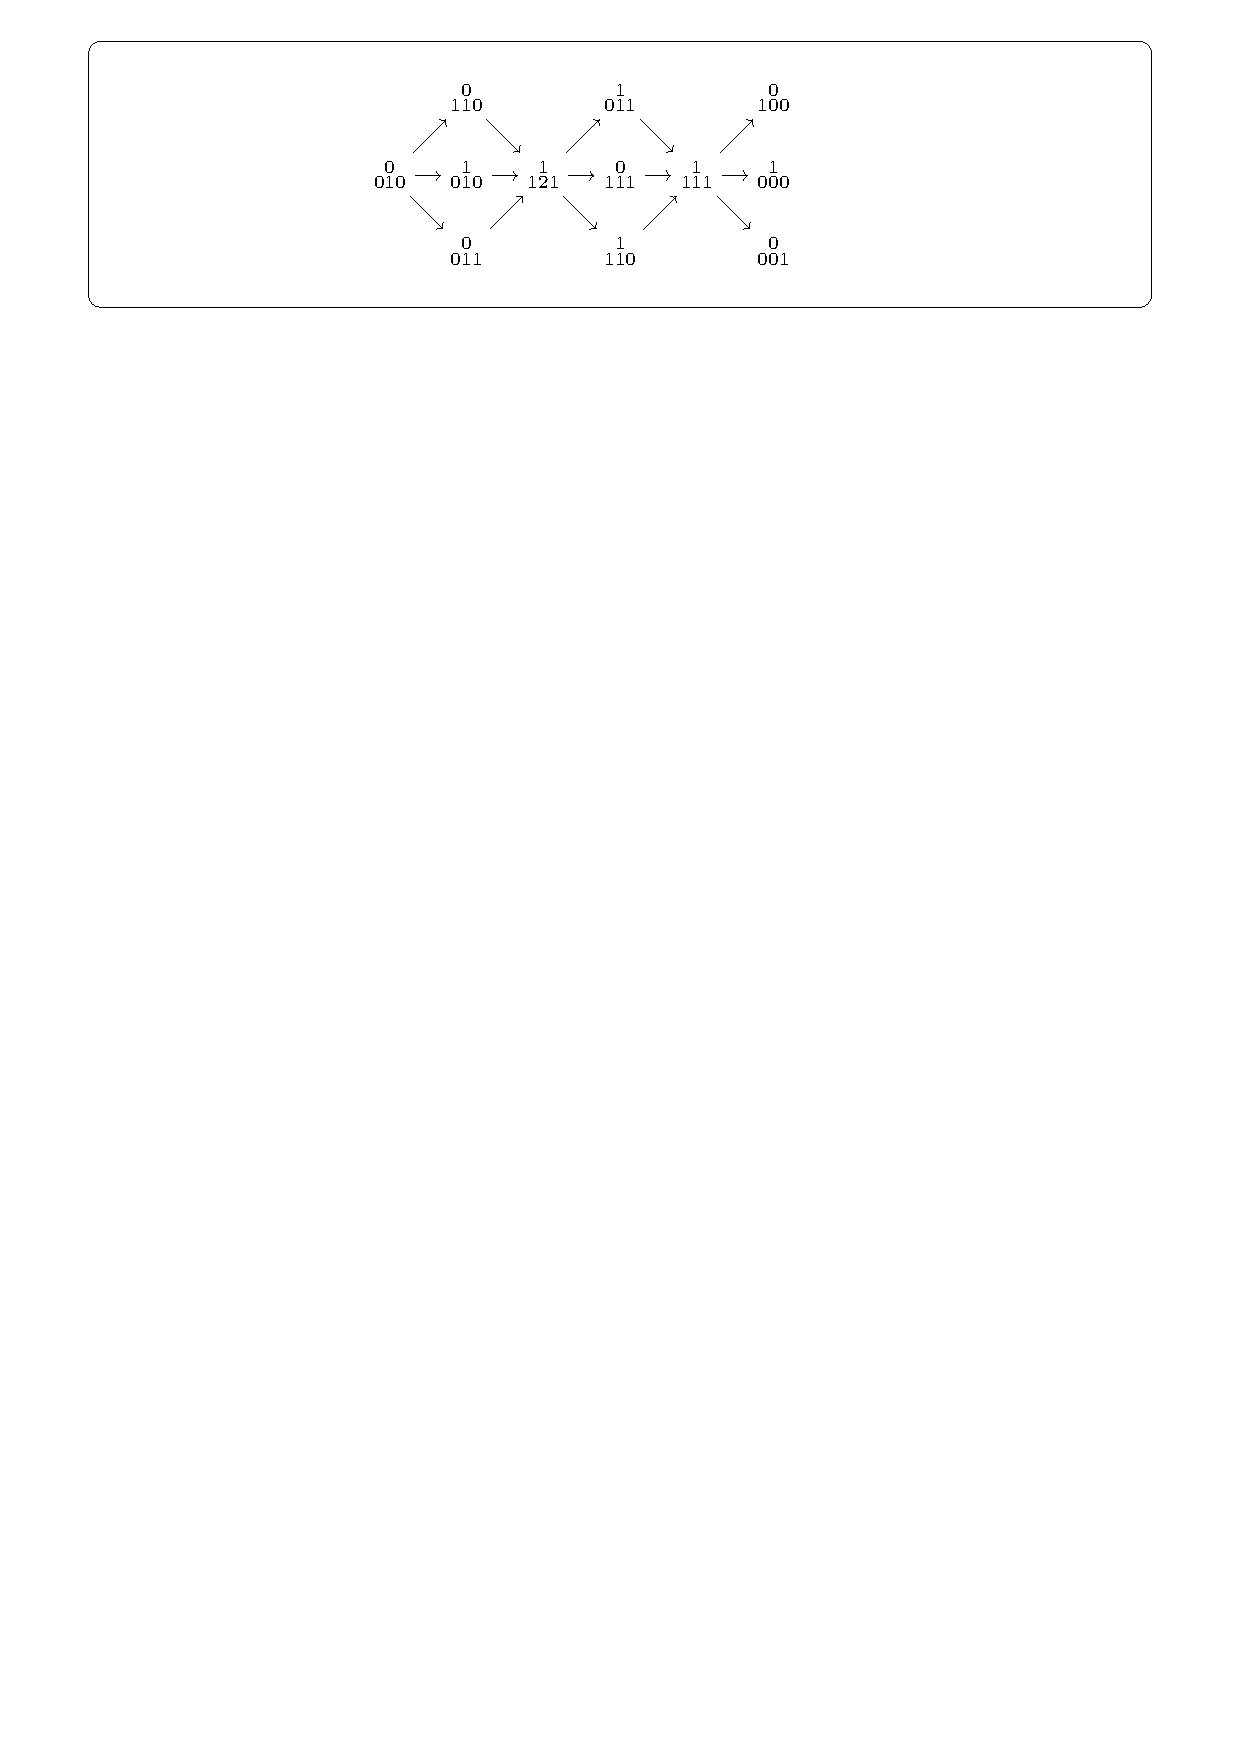
\includegraphics[clip, trim=1.1cm 22.5cm 1.1cm 0cm, width=1.00\textwidth]{figures/cardinput/card-final_noquiver.pdf}
}
\only<3>{
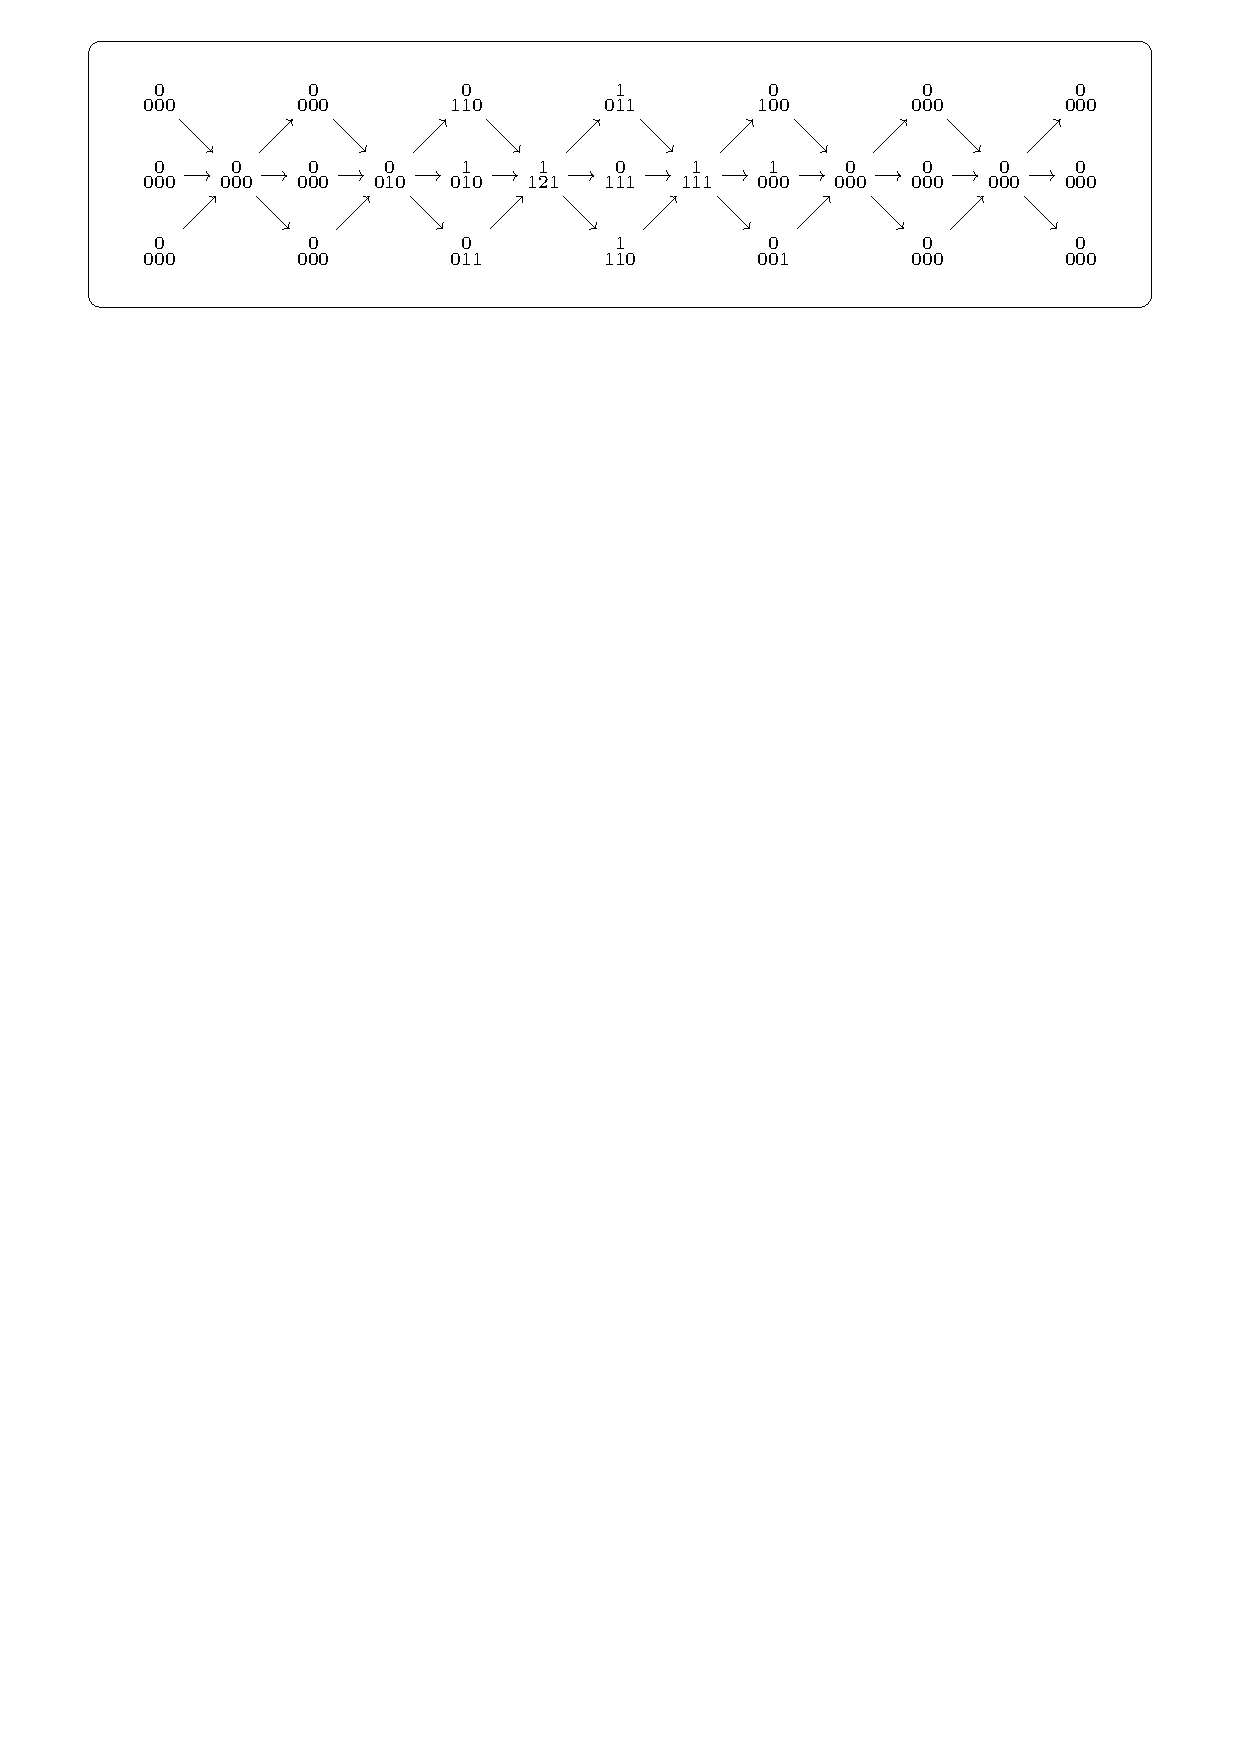
\includegraphics[clip, trim=1.1cm 22.5cm 1.1cm 0cm, width=1.00\textwidth]{figures/cardinput/card-final_noborder.pdf}
}
\only<4-5>{
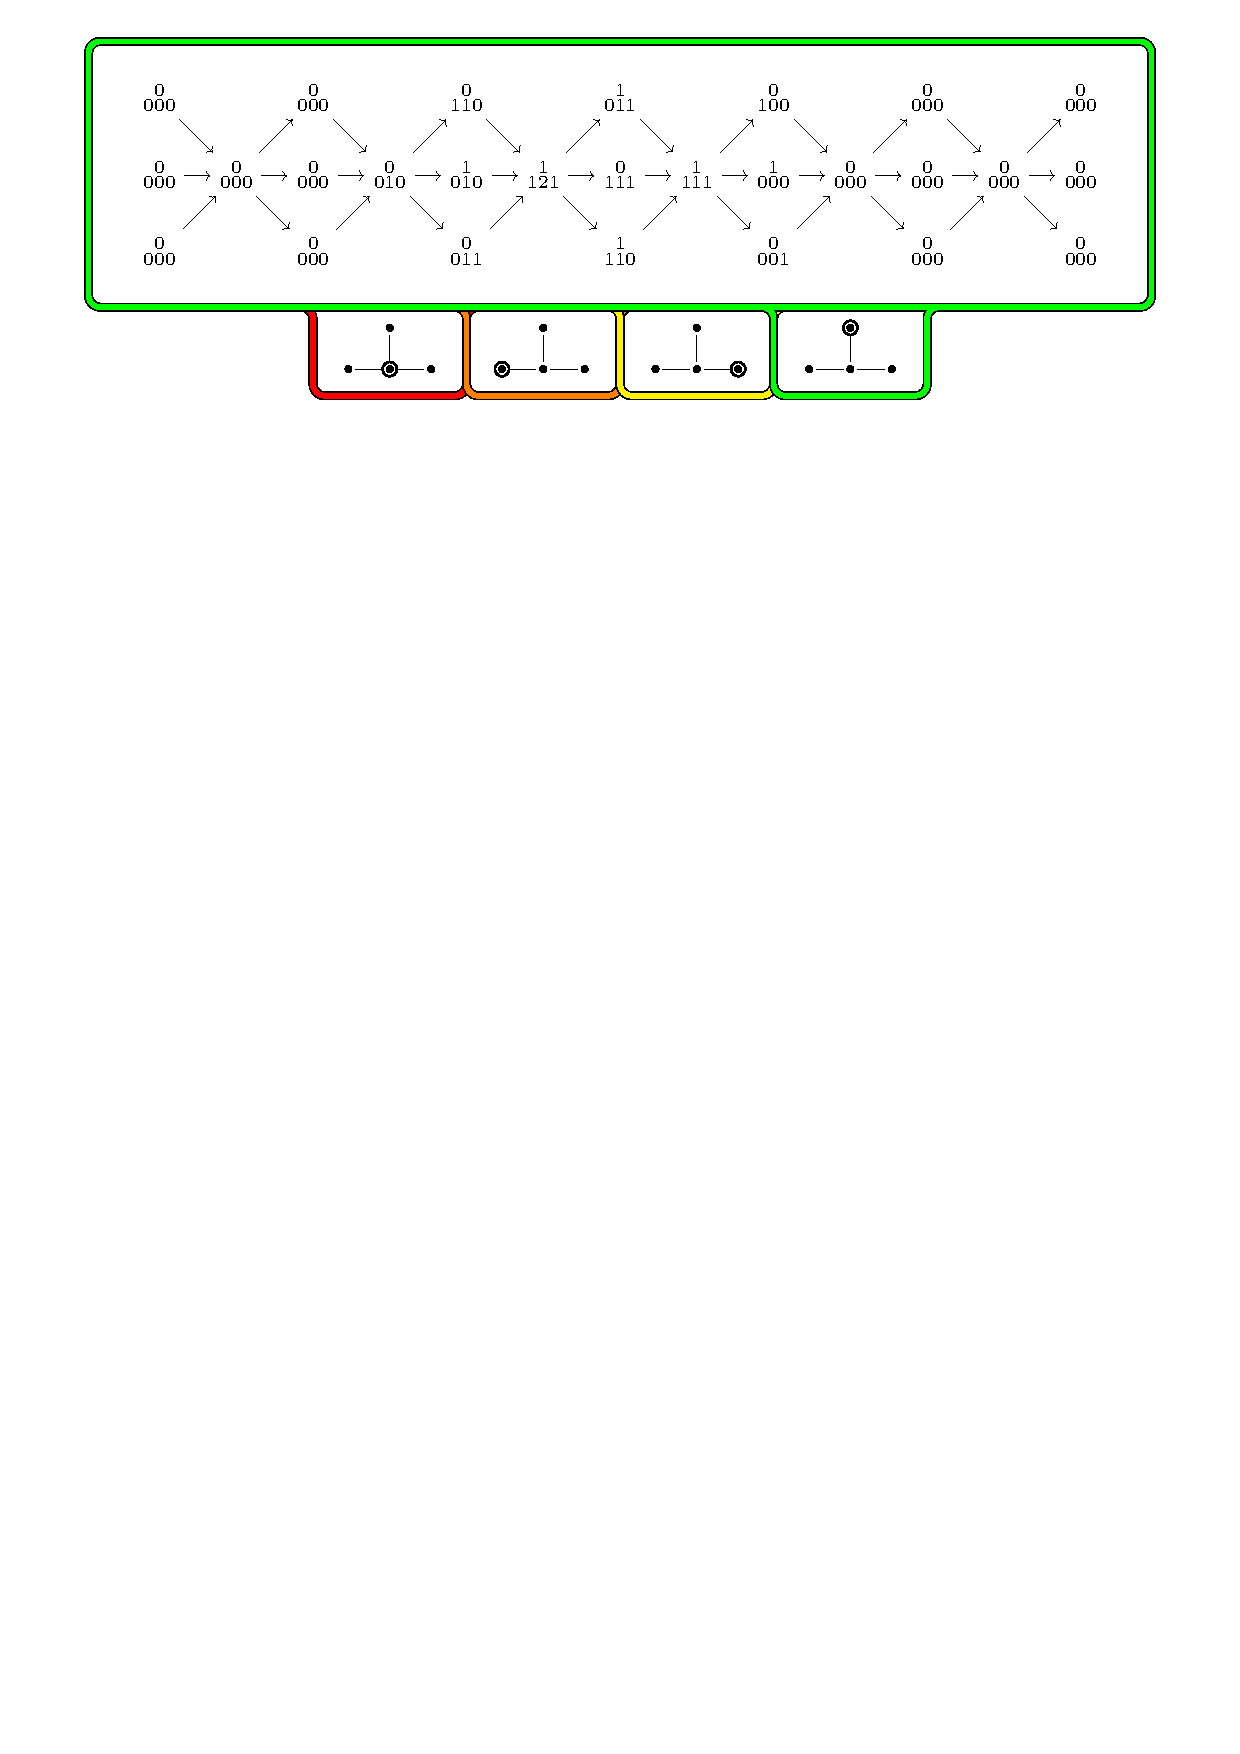
\includegraphics[clip, trim=1.1cm 22.5cm 1.1cm 0cm, width=1.00\textwidth]{figures/cardinput/card-final.pdf}
}
\end{short}

\only<1>{
\begin{short}
$$\text{ Shift cards } \quad \Longleftrightarrow \quad \text{ Switch arrows in $Q$ }$$
\end{short}
}
\only<5>{
\begin{short}
\href{http://home.ustc.edu.cn/~xx352229/webversion/webcard.html}{Interactive webversion}
\end{short}
}
\end{frame}



\begin{frame}[fragile]{Indecomposable representations of low order are easy!}


\begin{lemma}
Suppose $Q$ is a tree. For $M \in \ind(Q)$, $\ord(M) \leqslant 2$, 
$$\Flag_{\ftdimvec{f}}(M)\;\; \cong\quad \mathbb{P}^1 \times \cdots \times \mathbb{P}^1 \quad\text{ or }\quad \varnothing.$$
\end{lemma}

\begin{eg}
$\;\;Q= 
\adjustbox{scale=0.7}{
\begin{tikzcd}[sep={between origins, 10mm}, ampersand replacement=\&]
	\&\& \scriptstyle\bullet \&\\
	\scriptstyle\bullet \&\scriptstyle\bullet \& \scriptstyle\bullet \& \scriptstyle\bullet\\[-6mm]
	\arrow[from=1-3, to=2-3]
	\arrow[from=2-1, to=2-2]
	\arrow[from=2-3, to=2-2]
	\arrow[from=2-3, to=2-4]
\end{tikzcd}
}$  $ M
%=\substack{\phantom{1}1\\1221}
=\adjustbox{scale=0.68}{
\begin{tikzcd}[sep={between origins, 12mm}, ampersand replacement=\&]
	\&\& \mathbb{C} \&\\
	\mathbb{C} \&\mathbb{C}^2 \& \mathbb{C}^2 \& \mathbb{C}\\[-6mm]
	\arrow[hook,from=1-3, to=2-3]
	\arrow[hook,from=2-1, to=2-2]
	\arrow["\sim"',from=2-3, to=2-2]
	\arrow[two heads,from=2-3, to=2-4]
%	\arrow[from=1-3, to=2-3]
%	\arrow[from=2-1, to=2-2]
%	\arrow[from=2-3, to=2-2]
%	\arrow[from=2-3, to=2-4]
\end{tikzcd}
}$
%https://tex.stackexchange.com/questions/453436/how-to-make-large-brace-and-parenthesis-thinner
%https://tex.stackexchange.com/questions/385013/how-to-set-temporary-math-font
 $\rm \ftdimvec{f}= \left(\begin{smallmatrix}
&&0&\\
1&2&1&1\\[1mm]
&&0&\\
1&1&0&1\\
\end{smallmatrix}\right)$
\begin{equation*}
\begin{aligned}
  \Flag_{\ftdimvec{f}}(M)\hookrightarrow\;& \Flag_{\left(\substack{\scriptscriptstyle 1\\\scriptscriptstyle 1}\right)} (\mathbb{C}) \times 
  \Flag_{\left(\substack{\scriptscriptstyle 2\\\scriptscriptstyle 1}\right)} (\mathbb{C}^2) \times 
  \Flag_{\left(\substack{\scriptscriptstyle 1\\\scriptscriptstyle 0}\right)} (\mathbb{C}^2) \\
  \;& \times 
  \Flag_{\left(\substack{\scriptscriptstyle 1\\\scriptscriptstyle 1}\right)} (\mathbb{C}) \times 
  \Flag_{\left(\substack{\scriptscriptstyle 0\\\scriptscriptstyle 0}\right)} (\mathbb{C}) \\
   \;& \cong \mathbb{P}^1 \times \mathbb{P}^1
\end{aligned}
\end{equation*}



%% https://q.uiver.app/?q=WzAsOCxbMCwxLCJcXEZsYWdfe1xcZnRkaW12ZWN7Zn19KE0pIl0sWzEsMSwiXFxGbGFnX3tcXGxlZnQoXFxzdWJzdGFja3sxXFxcXDF9XFxyaWdodCl9IChcXG1hdGhiYntDfSkiXSxbMiwxLCJcXEZsYWdfe1xcbGVmdChcXHN1YnN0YWNrezJcXFxcMX1cXHJpZ2h0KX0gKFxcbWF0aGJie0N9XjIpIl0sWzMsMSwiXFxGbGFnX3tcXGxlZnQoXFxzdWJzdGFja3sxXFxcXDB9XFxyaWdodCl9IChcXG1hdGhiYntDfV4yKSJdLFszLDAsIlxcRmxhZ197XFxsZWZ0KFxcc3Vic3RhY2t7MFxcXFwwfVxccmlnaHQpfSAoXFxtYXRoYmJ7Q30pIl0sWzQsMSwiXFxGbGFnX3tcXGxlZnQoXFxzdWJzdGFja3sxXFxcXDF9XFxyaWdodCl9IChcXG1hdGhiYntDfSkiXSxbMSwyLCJcXG1hdGhiYntQfV4xIFxcdGltZXMgXFxtYXRoYmJ7UH1eMSJdLFswLDJdLFswLDEsIiIsMCx7InN0eWxlIjp7InRhaWwiOnsibmFtZSI6Imhvb2siLCJzaWRlIjoidG9wIn19fV0sWzEsMiwiXFx0aW1lcyIsMSx7InN0eWxlIjp7ImJvZHkiOnsibmFtZSI6Im5vbmUifSwiaGVhZCI6eyJuYW1lIjoibm9uZSJ9fX1dLFsyLDMsIlxcdGltZXMiLDEseyJzdHlsZSI6eyJib2R5Ijp7Im5hbWUiOiJub25lIn0sImhlYWQiOnsibmFtZSI6Im5vbmUifX19XSxbMyw1LCJcXHRpbWVzIiwxLHsic3R5bGUiOnsiYm9keSI6eyJuYW1lIjoibm9uZSJ9LCJoZWFkIjp7Im5hbWUiOiJub25lIn19fV0sWzQsMywiXFx0aW1lcyIsMSx7InN0eWxlIjp7ImJvZHkiOnsibmFtZSI6Im5vbmUifSwiaGVhZCI6eyJuYW1lIjoibm9uZSJ9fX1dLFs3LDYsIlxcY29uZyIsMSx7InN0eWxlIjp7ImJvZHkiOnsibmFtZSI6Im5vbmUifSwiaGVhZCI6eyJuYW1lIjoibm9uZSJ9fX1dXQ==
%\[\begin{tikzcd}[sep=tiny]
%	&&& {\Flag_{\left(\substack{0\\0}\right)} (\mathbb{C})} \\
%	{\Flag_{\ftdimvec{f}}(M)} & {\Flag_{\left(\substack{1\\1}\right)} (\mathbb{C})} & {\Flag_{\left(\substack{2\\1}\right)} (\mathbb{C}^2)} & {\Flag_{\left(\substack{1\\0}\right)} (\mathbb{C}^2)} & {\Flag_{\left(\substack{1\\1}\right)} (\mathbb{C})} \\
%	{} & {\mathbb{P}^1 \times \mathbb{P}^1}
%	\arrow[hook, from=2-1, to=2-2]
%	\arrow["\times"{description}, draw=none, from=2-2, to=2-3]
%	\arrow["\times"{description}, draw=none, from=2-3, to=2-4]
%	\arrow["\times"{description}, draw=none, from=2-4, to=2-5]
%	\arrow["\times"{description}, draw=none, from=1-4, to=2-4]
%	\arrow["\cong"{description}, draw=none, from=3-1, to=3-2]
%\end{tikzcd}\]
\end{eg}

\end{frame}

\begin{frame}[fragile]{Continue}


% Please add the following required packages to your document preamble:
% \usepackage{multirow}

\newcolumntype{Y}{>{\centering\arraybackslash}X}
\newcolumntype{L}{>{$}Y<{$}} % math-mode version 
\begin{table}[]

\[
\begin{tabularx}{.78\textwidth}{|c|*{6}{L|}}
\hline
 & \multicolumn{2}{c|}{$\mathbb{C} \hookrightarrow \mathbb{C}^2$} & \multicolumn{2}{c|}{$\mathbb{C}^2 \twoheadrightarrow \mathbb{C}$} & \multicolumn{2}{c|}{$\mathbb{C}^2 \rightarrow \mathbb{C}^2$} \\
 \hline
\multirow{2}{*}{No restriction} & - & 2 & 0 & - & - & 1 \\
\cline{2-7}
 & 0 & - & 1 & 2 & 0 & 0 \\
 \hline
Reduce & 1 & 1 & 1 & 1 & 1 & 0 \\
\hline
\multirow{3}{*}{Impossible} & 2 & 1 &  &  &  &  \\
\cline{2-3}
 & 2 & 0 & 1 & 0 & 2 & 0 \\\cline{2-3}
 & 1 & 0 &  &  &  &  \\\hline
\end{tabularx}
\]
\end{table}



\begin{corollary}
The main theorem is true for quivers of type $A$, $D$.
\end{corollary}
\end{frame}



%%%%%%%%%%%%%%%%%%%%%%%%%%%%%%%%%%%%%%%%%%%%%%%
\section{Tackle the type $E$ case}
\begin{frame}{Process}
\tableofcontents[currentsection,hideallsubsections]
\end{frame}

\begin{frame}[fragile]{Process}
\begin{figure}[ht]
    \centering
    \only<1>{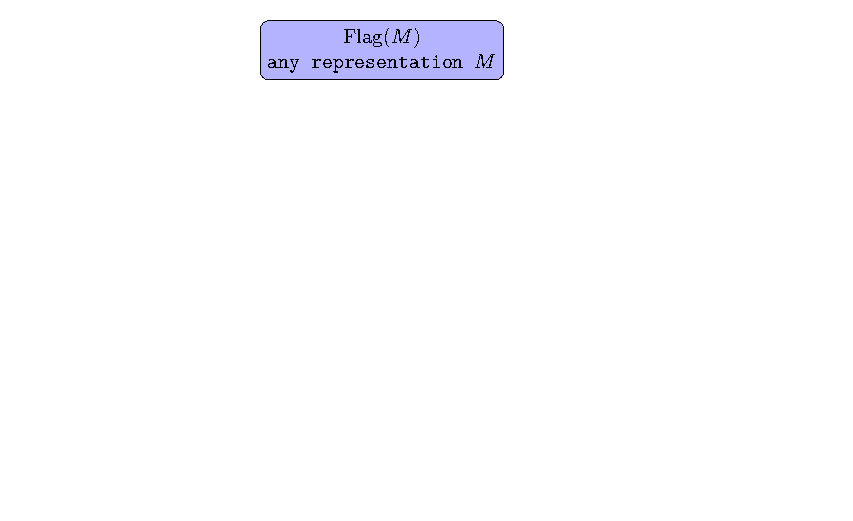
\includegraphics[scale=0.75]{figures/flowchart/flowchart11.pdf}}
    \only<2>{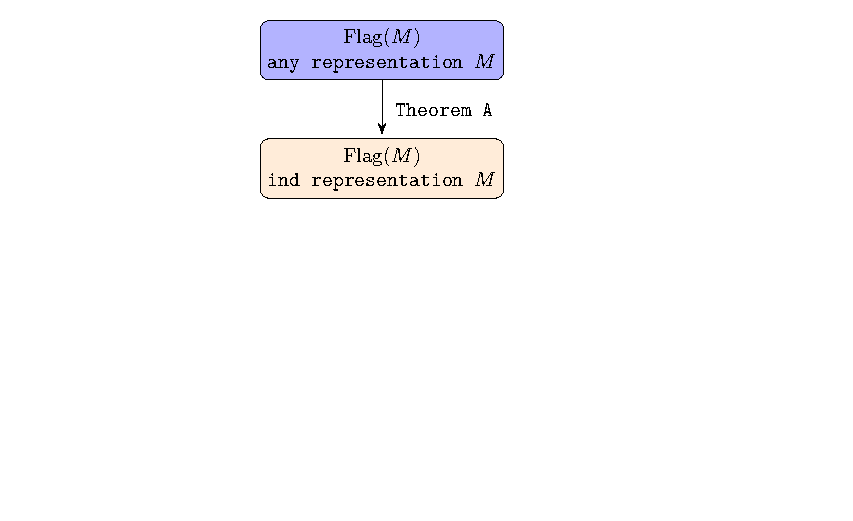
\includegraphics[scale=0.75]{figures/flowchart/flowchart12.pdf}}
    \only<3>{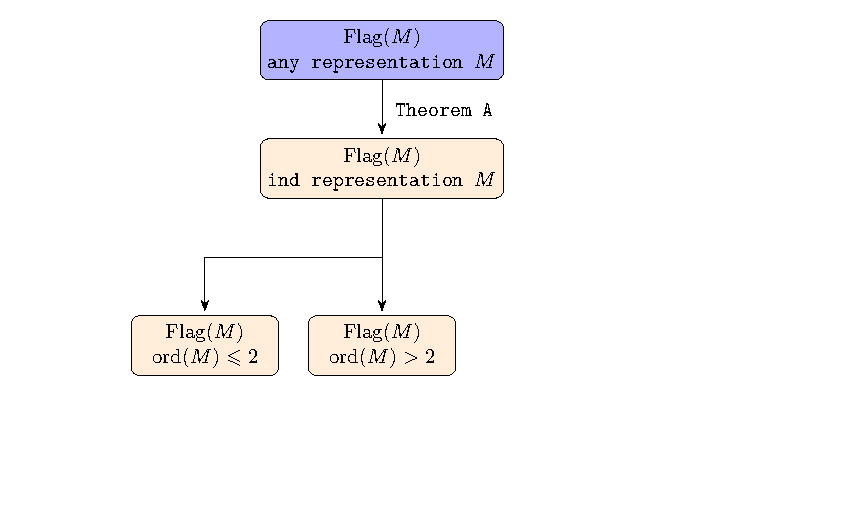
\includegraphics[scale=0.75]{figures/flowchart/flowchart13.pdf}}
    \only<4>{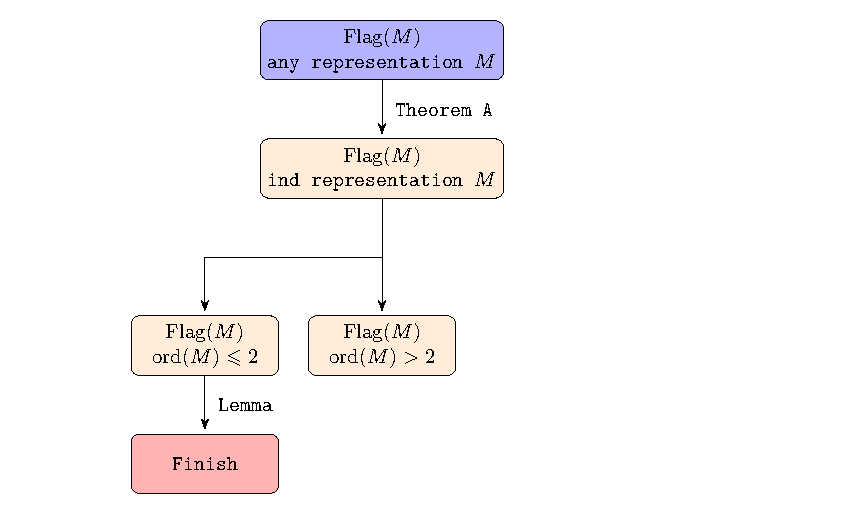
\includegraphics[scale=0.75]{figures/flowchart/flowchart1.pdf}}
%    \only<5>{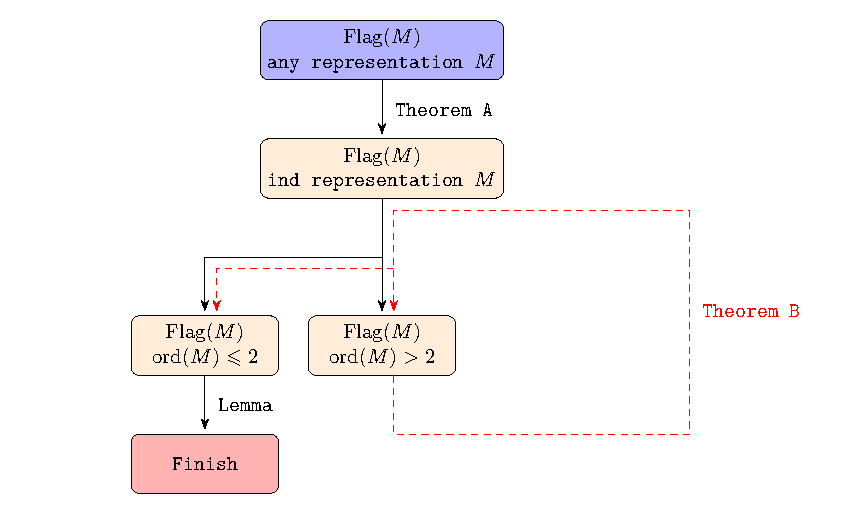
\includegraphics[scale=0.75]{figures/flowchart/flowchart2.pdf}}
%    \only<6>{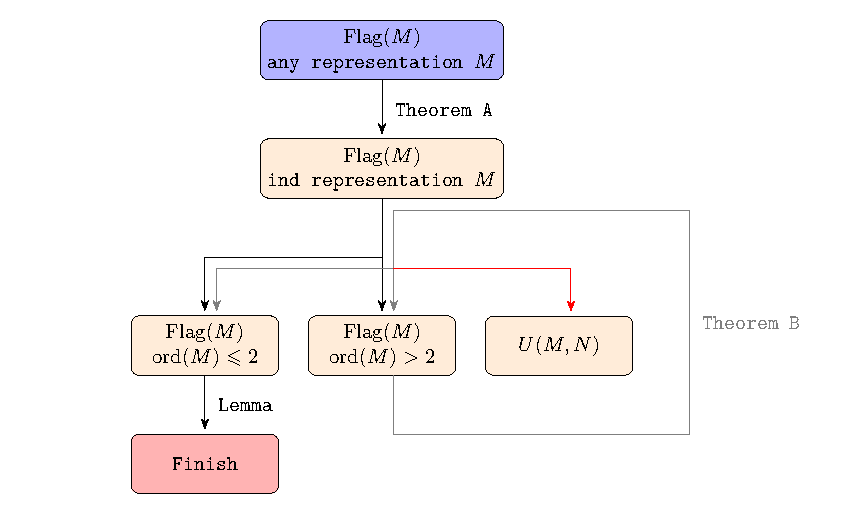
\includegraphics[scale=0.75]{figures/flowchart/flowchart3.pdf}}
%    \only<7>{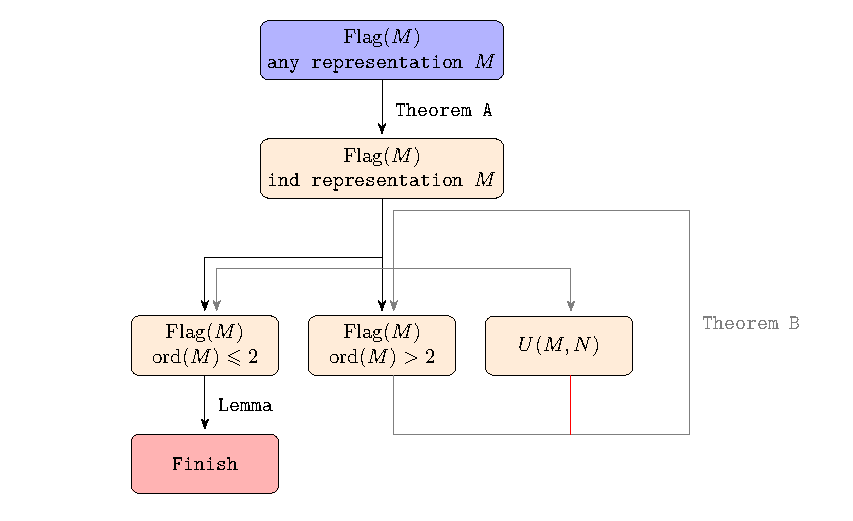
\includegraphics[scale=0.75]{figures/flowchart/flowchart4.pdf}}
\end{figure}
\end{frame}

\begin{frame}[fragile]{What is remaining?}
\begin{flushleft}

      $E_6$ :\parbox[h][][c]{7cm}{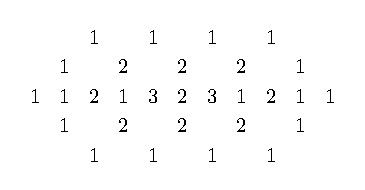
\includegraphics[height=0.28\textheight]{figures/horizontal/h_E6.pdf}}
      \\[-2mm]
      $E_7$ :\parbox[h][][c]{7cm}{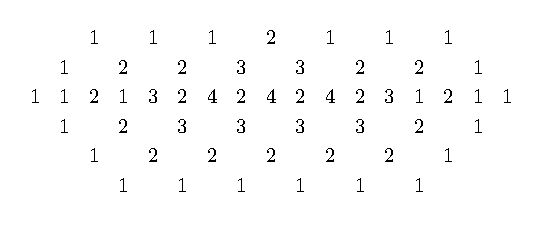
\includegraphics[height=0.32\textheight]{figures/horizontal/h_E7.pdf}}
      \\[-7mm]
      $E_8$ :\parbox[h][][c]{7cm}{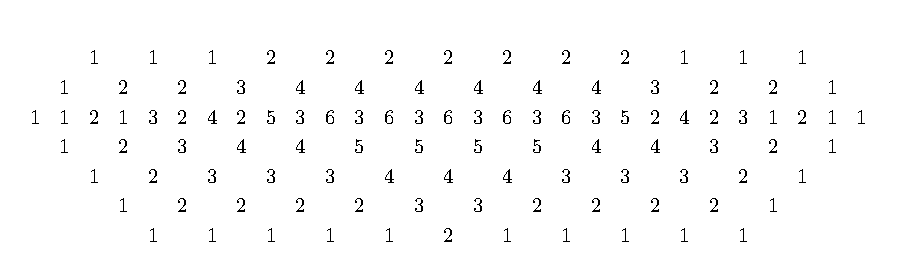
\includegraphics[height=0.37\textheight]{figures/horizontal/h_E8.pdf}}
\end{flushleft}
\end{frame}

\begin{frame}[fragile]{What is remaining?}
\begin{flushleft}

      $E_6$ :\parbox[h][][c]{7cm}{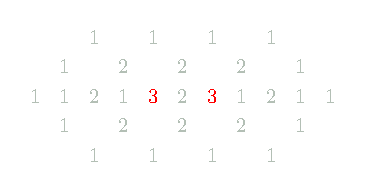
\includegraphics[height=0.28\textheight]{figures/horizontal/h_E6_red.pdf}}
      \\[-2mm]
      $E_7$ :\parbox[h][][c]{7cm}{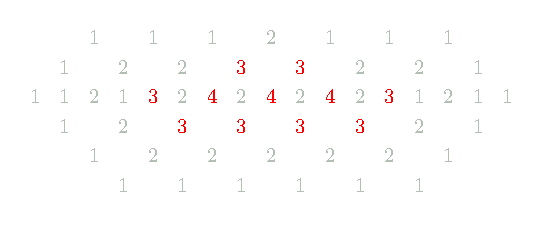
\includegraphics[height=0.32\textheight]{figures/horizontal/h_E7_red.pdf}}
      \\[-7mm]
      $E_8$ :\parbox[h][][c]{7cm}{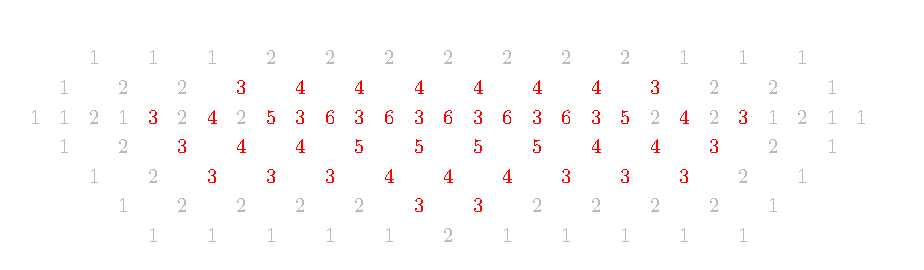
\includegraphics[height=0.37\textheight]{figures/horizontal/h_E8_red.pdf}}
\end{flushleft}
\end{frame}

\begin{frame}[fragile]{Process}
\begin{figure}[ht]
    \centering
    \only<1>{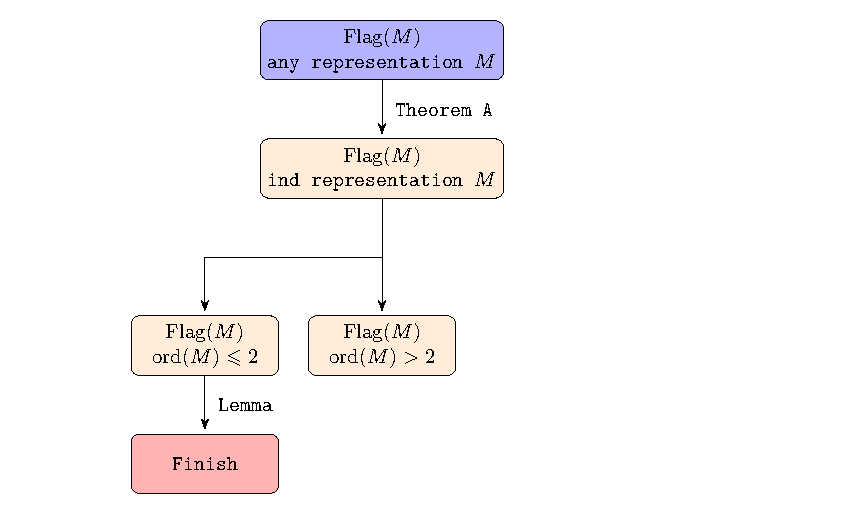
\includegraphics[scale=0.75]{figures/flowchart/flowchart1.pdf}}
    \only<2>{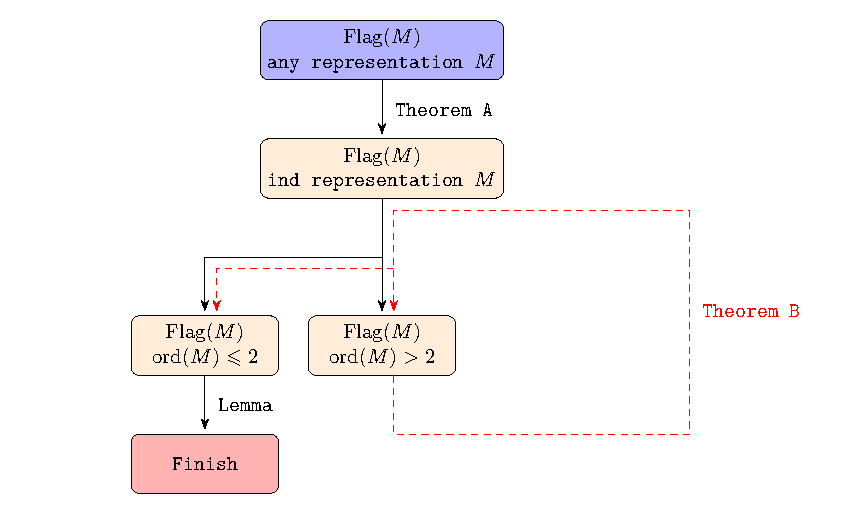
\includegraphics[scale=0.75]{figures/flowchart/flowchart2.pdf}}
\end{figure}
\end{frame}

\begin{frame}[fragile]
\noindent Consider the short exact sequence of representations
\vspace{-3mm}
\[\begin{tikzcd}
\eta: 0 & {X} & {Y} & {S} & 0
\arrow[from=1-1, to=1-2]
\arrow["\iota", from=1-2, to=1-3]
\arrow["\pi", from=1-3, to=1-4]
\arrow[from=1-4, to=1-5]
\end{tikzcd}\]

\vspace{-4mm}
\noindent which induce maps
\vspace{-4mm}
% https://q.uiver.app/?q=WzAsNixbMSwwLCIgXFxGbGFnX2QoWSkiXSxbMiwwLCJcXEZsYWdfZChYKSBcXHRpbWVzIFxcRmxhZ19kKFMpIl0sWzEsMSwiXFxGbGFnKFkpX3tcXGZ0ZGltdmVje2Z9LFxcZnRkaW12ZWN7Z319Il0sWzIsMSwiXFxGbGFnX3tcXGZ0ZGltdmVje2Z9fShYKSBcXHRpbWVzIFxcRmxhZ197XFxmdGRpbXZlY3tnfX0oUykiXSxbMCwwLCJcXFBzaToiXSxbMCwxLCJcXFBzaV97XFxmdGRpbXZlY3tmfSxcXGZ0ZGltdmVje2d9fTogIl0sWzIsM10sWzAsMV0sWzIsMCwiXFxzdWJzZXQiLDEseyJzdHlsZSI6eyJib2R5Ijp7Im5hbWUiOiJub25lIn0sImhlYWQiOnsibmFtZSI6Im5vbmUifX19XSxbMywxLCJcXHN1YnNldCIsMSx7InN0eWxlIjp7ImJvZHkiOnsibmFtZSI6Im5vbmUifSwiaGVhZCI6eyJuYW1lIjoibm9uZSJ9fX1dXQ==
\[\begin{tikzcd}[row sep={1mm}]
	{\phantom{f,g}\Psi:} &[-10mm] { \Flag_d(Y)} & {\Flag_d(X) \times \Flag_d(S)} \\
	{\Psi_{\ftdimvec{f},\ftdimvec{g}}: } & {\Flag(Y)_{\ftdimvec{f},\ftdimvec{g}}} & {\Flag_{\ftdimvec{f}}(X) \times \Flag_{\ftdimvec{g}}(S)}
	\arrow[from=2-2, to=2-3]
	\arrow[from=1-2, to=1-3]
	\arrow["\subset"{description}, sloped, draw=none, from=2-2, to=1-2]
	\arrow["\subset"{description}, sloped, draw=none, from=2-3, to=1-3]
\end{tikzcd}\]
\vspace{-6mm}
\begin{block}{Theorem B}
When $\eta$ does not split and generates $\Ext^1(S,X)$, 
\vspace{-2mm}
\begin{center}
$\Psi_{\ftdimvec{f},\ftdimvec{g}}$ is a Zarisky-locally trivial affine bundle over $\Img \Psi_{\ftdimvec{f},\ftdimvec{g}}$.
\end{center}
\vspace{-2mm}
In this case, we have a clear description of $\Img \Psi_{\ftdimvec{f},\ftdimvec{g}}$.
\end{block}
\end{frame}






\begin{frame}[fragile,t]{How to find nice $\eta$?}

%\begin{overlayarea}{\linewidth}{\textheight}
\begin{proposition}
For $X \hookrightarrow Y$ \textcolor{red}{irreducible mono}, the induced SES
\vspace{-3mm}
\[\begin{tikzcd}
\eta: 0 & {X} & {Y} & {S} & 0
\arrow[from=1-1, to=1-2]
\arrow["\iota", from=1-2, to=1-3]
\arrow["\pi", from=1-3, to=1-4]
\arrow[from=1-4, to=1-5]
\end{tikzcd}\]
\\
\vspace{-3mm}
satisfies the condition of Theorem B. Moreover,
\vspace{-3mm}
\only<1-2>{$$\Img \Psi_{\ftdimvec{f},\ftdimvec{g}} = \begin{cases}
\left(\Flag_{\ftdimvec{f}}(X) \smallsetminus \Flag_{\ftdimvec{f}}(X_S)\right) \times \Flag_{\ftdimvec{g}}(S), & \ftdimvec{g}_i=\dimv S\\
\;\Flag_{\ftdimvec{f}}(X) \times \Flag_{\ftdimvec{g}}(S), & \text{otherwise}
\end{cases}$$}
\only<3>{$$\Img \Psi_{\ftdimvec{f},\ftdimvec{g}} = \begin{cases}
\;U_{\ftdimvec{f}}(X,X_S), & \ftdimvec{g}_i=\dimv S\\
\;\Flag_{\ftdimvec{f}}(X) \times \Flag_{\ftdimvec{g}}(S),\hspace{15mm}$\,$ & \text{otherwise}
\end{cases}$$}
\\
\vspace{-3mm}
\only<1>{where
\vspace{-3mm}
$$X_S:= \max \left\{ M \subseteq X \,\middle|\; \Ext^1(S,X/M) \cong \mathbb{C} \right\} \subseteq X.$$}
\end{proposition}
\only<2-3>{
\begin{figure}[ht]
  \vspace{-0.3cm}
    \centering  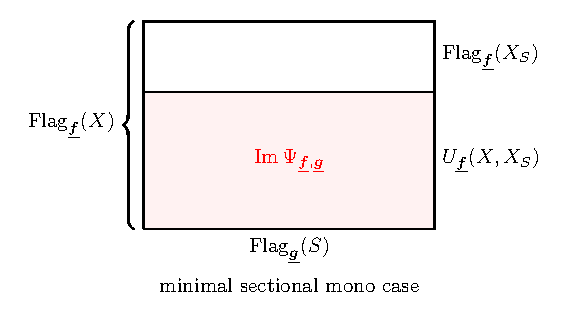
\includegraphics[width=6cm]{figures/space/preferredimage.pdf}
       \end{figure} 
}
%\end{overlayarea}
\end{frame}

\begin{frame}[fragile]{Process}
\begin{figure}[ht]
    \centering
    \only<1>{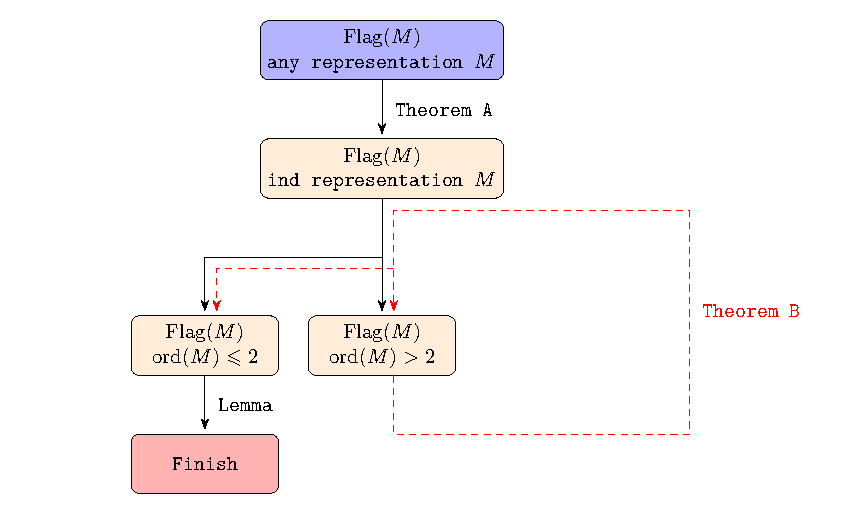
\includegraphics[scale=0.75]{figures/flowchart/flowchart2.pdf}}
    \only<2>{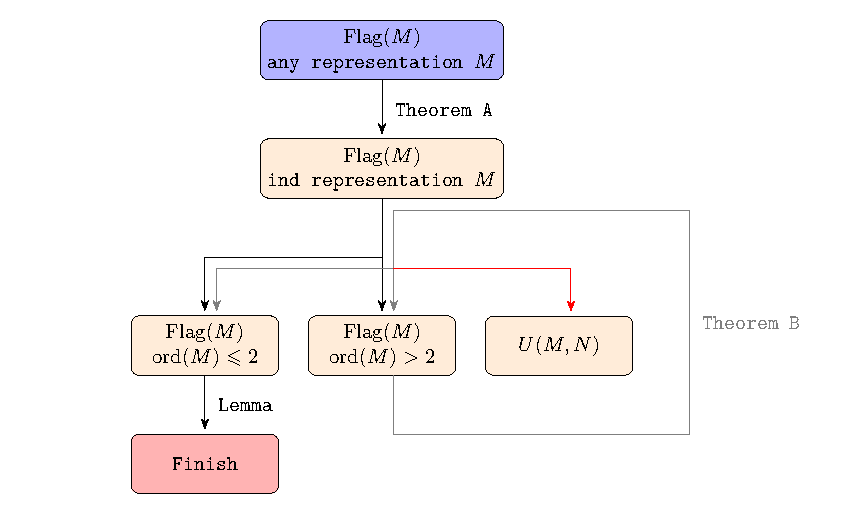
\includegraphics[scale=0.75]{figures/flowchart/flowchart3.pdf}}
\end{figure}
\end{frame}

\begin{frame}[fragile,t]{Induction?}
\begin{proposition}
For $X \hookrightarrow Y$ irreducible mono, the induced SES
\vspace{-3mm}
\[\begin{tikzcd}
\eta: 0 & {X} & {Y} & {S} & 0
\arrow[from=1-1, to=1-2]
\arrow["\iota", from=1-2, to=1-3]
\arrow["\pi", from=1-3, to=1-4]
\arrow[from=1-4, to=1-5]
\end{tikzcd}\]
\\
\vspace{-3mm}
satisfies the condition of Theorem B. Moreover,
\vspace{-3mm}
$$\Img \Psi_{\ftdimvec{f},\ftdimvec{g}} = \begin{cases}
U_{\ftdimvec{f}}(X,X_S), & \ftdimvec{g}_i=\dimv S\\
\;\Flag_{\ftdimvec{f}}(X) \times \Flag_{\ftdimvec{g}}(S),\hspace{15mm}$\,$ & \text{otherwise}
\end{cases}$$

\end{proposition}
\begin{proposition}
In addition,\\[-5mm]
$$X_S=0 \quad \text{ or } \quad X_S \hookrightarrow X \text{ is irreducible mono.}$$
\end{proposition}

\begin{corollary}
For $M \in \ind(Q)$, if exist irreducible mono $X \hookrightarrow M$, then\\[-5mm]
$$\Flag_{d}(M) \text{ has an affine paving.}$$
\end{corollary}
\end{frame}

\begin{frame}[fragile]{Process}
\begin{figure}[ht]
    \centering
%    \only<1>{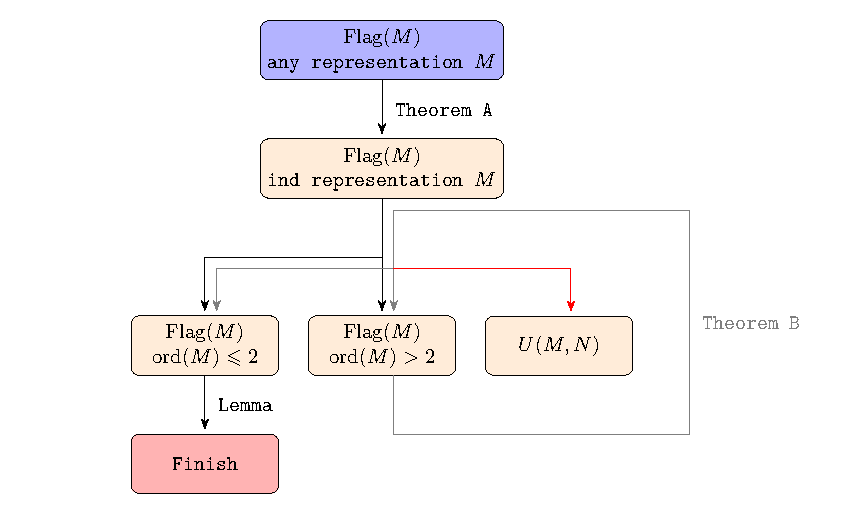
\includegraphics[scale=0.75]{figures/flowchart/flowchart3.pdf}}
    \only<1>{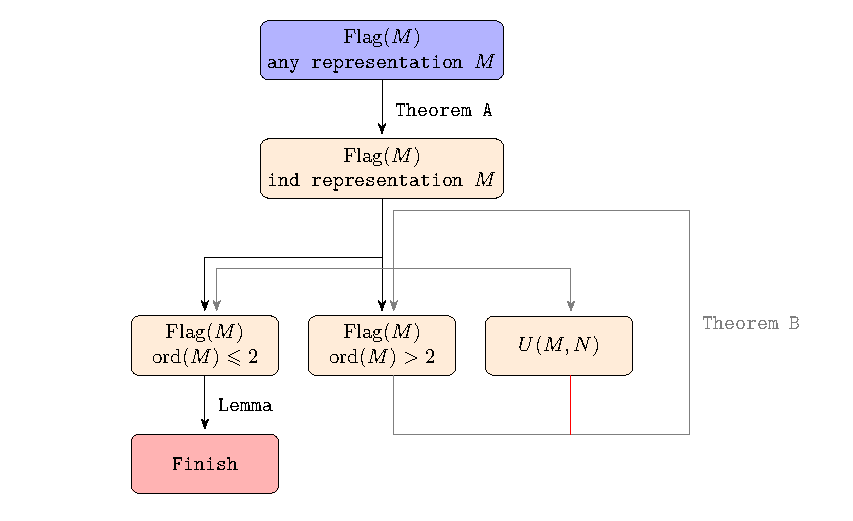
\includegraphics[scale=0.75]{figures/flowchart/flowchart4.pdf}}
    \label{fig:flowchart}
\end{figure}
\end{frame}


%\begin{frame}[fragile]{What is remaining?}
%\begin{flushleft}
%
%      $E_6$ :\parbox[h][][c]{7cm}{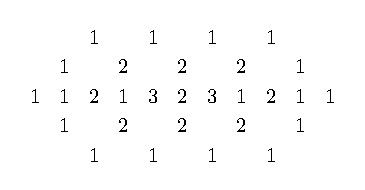
\includegraphics[height=0.28\textheight]{figures/horizontal/h_E6.pdf}}
%      \\[-2mm]
%      $E_7$ :\parbox[h][][c]{7cm}{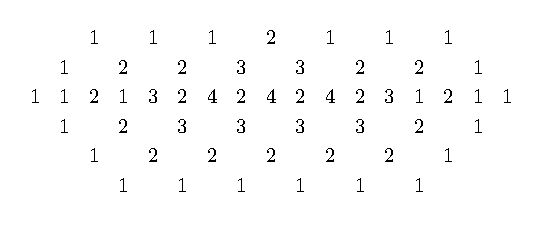
\includegraphics[height=0.32\textheight]{figures/horizontal/h_E7.pdf}}
%      \\[-7mm]
%      $E_8$ :\parbox[h][][c]{7cm}{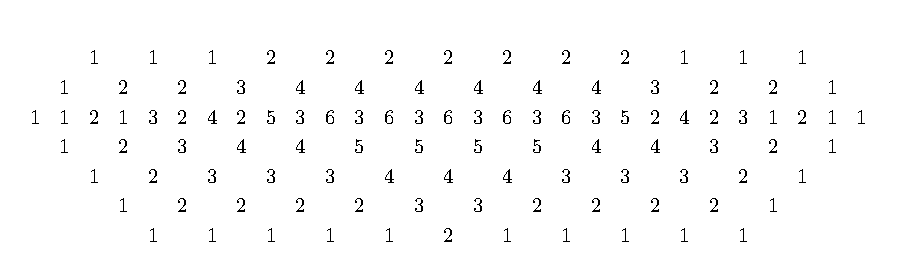
\includegraphics[height=0.37\textheight]{figures/horizontal/h_E8.pdf}}
%\end{flushleft}
%\end{frame}

\begin{frame}[fragile]{What is remaining?}
\begin{flushleft}

      $E_6$ :\parbox[h][][c]{7cm}{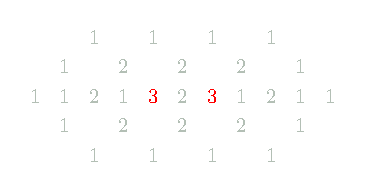
\includegraphics[height=0.28\textheight]{figures/horizontal/h_E6_red.pdf}}
      \\[-2mm]
      $E_7$ :\parbox[h][][c]{7cm}{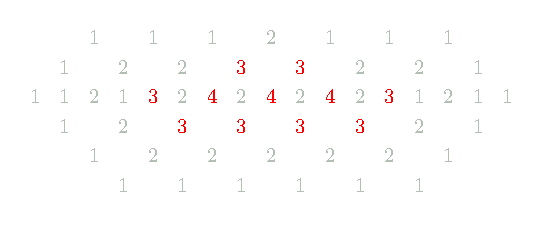
\includegraphics[height=0.32\textheight]{figures/horizontal/h_E7_red.pdf}}
      \\[-7mm]
      $E_8$ :\parbox[h][][c]{7cm}{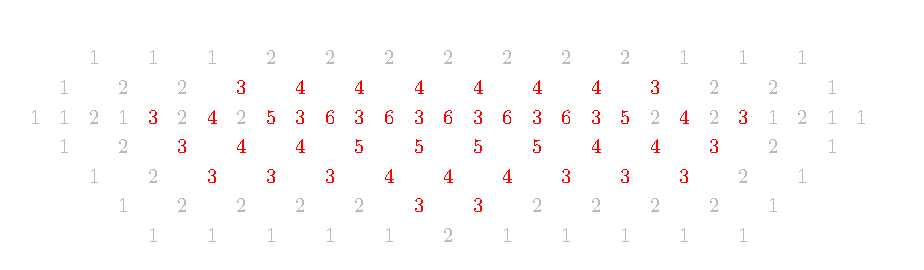
\includegraphics[height=0.37\textheight]{figures/horizontal/h_E8_red.pdf}}
\end{flushleft}
\end{frame}
\begin{frame}[fragile]{What is remaining?}
\begin{flushleft}

      $E_6$ :\parbox[h][][c]{7cm}{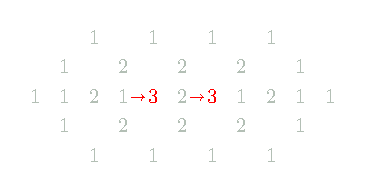
\includegraphics[height=0.28\textheight]{figures/horizontal/h_E6_red_easy.pdf}}
      \\[-2mm]
      $E_7$ :\parbox[h][][c]{7cm}{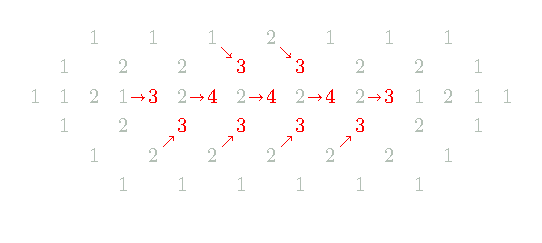
\includegraphics[height=0.32\textheight]{figures/horizontal/h_E7_red_easy.pdf}}
      \\[-7mm]
      $E_8$ :\parbox[h][][c]{7cm}{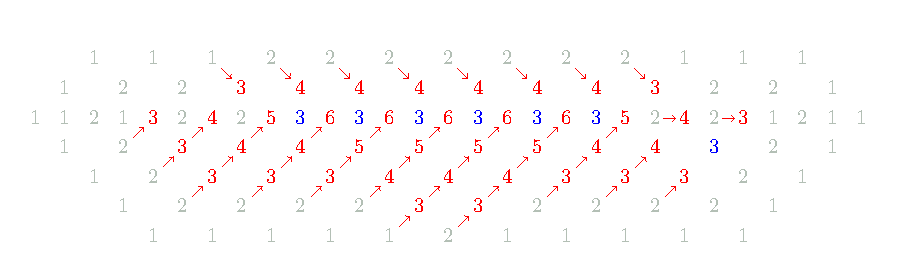
\includegraphics[height=0.37\textheight]{figures/horizontal/h_E8_red_easy.pdf}}
\end{flushleft}
\end{frame}
\begin{frame}[fragile]{What is remaining?}
\begin{flushleft}

      $E_6$ :\parbox[h][][c]{7cm}{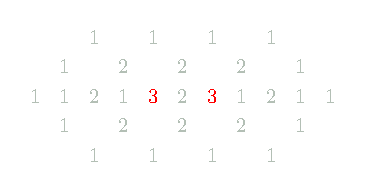
\includegraphics[height=0.28\textheight]{figures/horizontal/h_E6_red.pdf}}
      \\[-2mm]
      $E_7$ :\parbox[h][][c]{7cm}{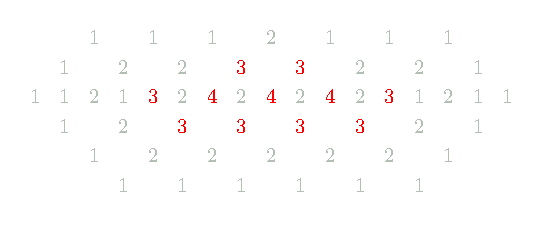
\includegraphics[height=0.32\textheight]{figures/horizontal/h_E7_red.pdf}}
      \\[-7mm]
      $E_8$ :\parbox[h][][c]{7cm}{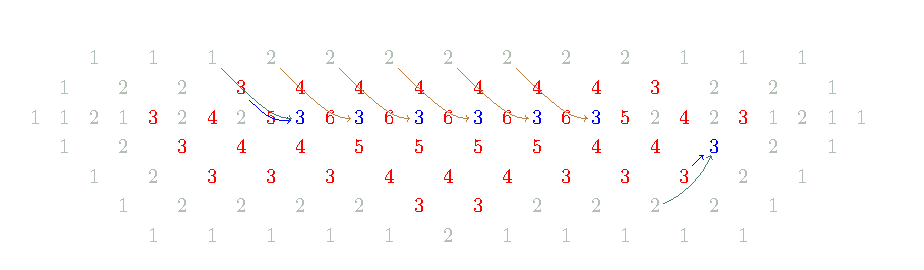
\includegraphics[height=0.37\textheight]{figures/horizontal/h_E8_red_hard.pdf}}
\end{flushleft}
\end{frame}


\begin{frame}[fragile]{Q \& A}
Thank you! Any questions?
\end{frame}





\end{document}